\documentclass[conference]{IEEEtran}
\IEEEoverridecommandlockouts
% The preceding line is only needed to identify funding in the first footnote. If that is unneeded, please comment it out.
\usepackage{cite}
\usepackage{amsmath,amssymb,amsfonts}
\usepackage{algorithmic}
\usepackage{graphicx}
\usepackage{textcomp}
\usepackage{xcolor}
\usepackage[T1]{fontenc}
\usepackage{newtxtext,newtxmath}
\usepackage{subfig}  % Enables subfigures for better layout
\usepackage{float}    % Allows [H] for strict placement
\usepackage{comment}
\usepackage{url}
\usepackage{multirow}
\usepackage{booktabs}
\usepackage[table]{xcolor}
\usepackage{colortbl}
\usepackage{array}
\usepackage{makecell}
\renewcommand{\bfdefault}{b}
\graphicspath{{./figures}}
\def\BibTeX{{\rm B\kern-.05em{\sc i\kern-.025em b}\kern-.08em
		T\kern-.1667em\lower.7ex\hbox{E}\kern-.125emX}}
\begin{document}
	
	\title{Multi-Floor IPS, a Simplified Indoor Positioning System Study*\\
		{\footnotesize \textsuperscript{*}Note: Sub-titles are not captured in Xplore and
			should not be used}
		\thanks{Identify applicable funding agency here. If none, delete this.}
	}
	
	\author{\IEEEauthorblockN{1\textsuperscript{st} Given Name Surname}
		\IEEEauthorblockA{\textit{dept. name of organization (of Aff.)} \\
			\textit{name of organization (of Aff.)}\\
			City, Country \\
			email address or ORCID}
		\and
		\IEEEauthorblockN{2\textsuperscript{nd} Given Name Surname}
		\IEEEauthorblockA{\textit{dept. name of organization (of Aff.)} \\
			\textit{name of organization (of Aff.)}\\
			City, Country \\
			email address or ORCID}
		\and
		\IEEEauthorblockN{3\textsuperscript{rd} Given Name Surname}
		\IEEEauthorblockA{\textit{dept. name of organization (of Aff.)} \\
			\textit{name of organization (of Aff.)}\\
			City, Country \\
			email address or ORCID}
	}
	
	\maketitle
	
	\begin{abstract}
		Indoor positioning systems are a relatively new positioning tool that aims to supplement or replace the usage of Global Positioning Tools for indoor positioning. However; there are minimal studies on Indoor positioning systems in a multi-floor model. This paper aims to provide further knowledge on multi-floor indoor positioning models through demonstrating and analyzing the process of creating a multi-floor indoor positioning model, analysis of machine learning models and how well they perform in a multi-floor indoor positioning model. This paper also aims to introduce two new metrics, Average Grid from Target and Average Distance from Target to better quantify IPS performance as well as the effects of feature filtering, grid size, and data point density on positioning accuracy. The paper also demonstrates the effects of varying grid size on the machine learning model, through Average Grid from Target (AGT). The experiment was conducted on the 6th and 7th floor hallways of an university learning center. With each part of the hallway being segmented into 1x1 metre grids. Two Android devices running a modified open-source IPS data collection application were used to gather RSSI data across approximately 600 grids per floor. A dataset of 12,640 points was collected across two floors using a filtered set of 378 BSSIDs containing specific identifiers Experiments with different grid sizes showed that different parameter settings are better for optimizing solely for accuracy or for Average Grid from Target (AGT). The study concludes that a 7×7m grid size offers the best balance between accuracy and precision for IPS applications. A simple WiFi access points filter was implemented. It lowered training time, computational load as well as slightly improved model stability. 
	\end{abstract}
	
	\begin{IEEEkeywords}
		component, formatting, style, styling, insert
	\end{IEEEkeywords}
	
	\begin{figure*}
		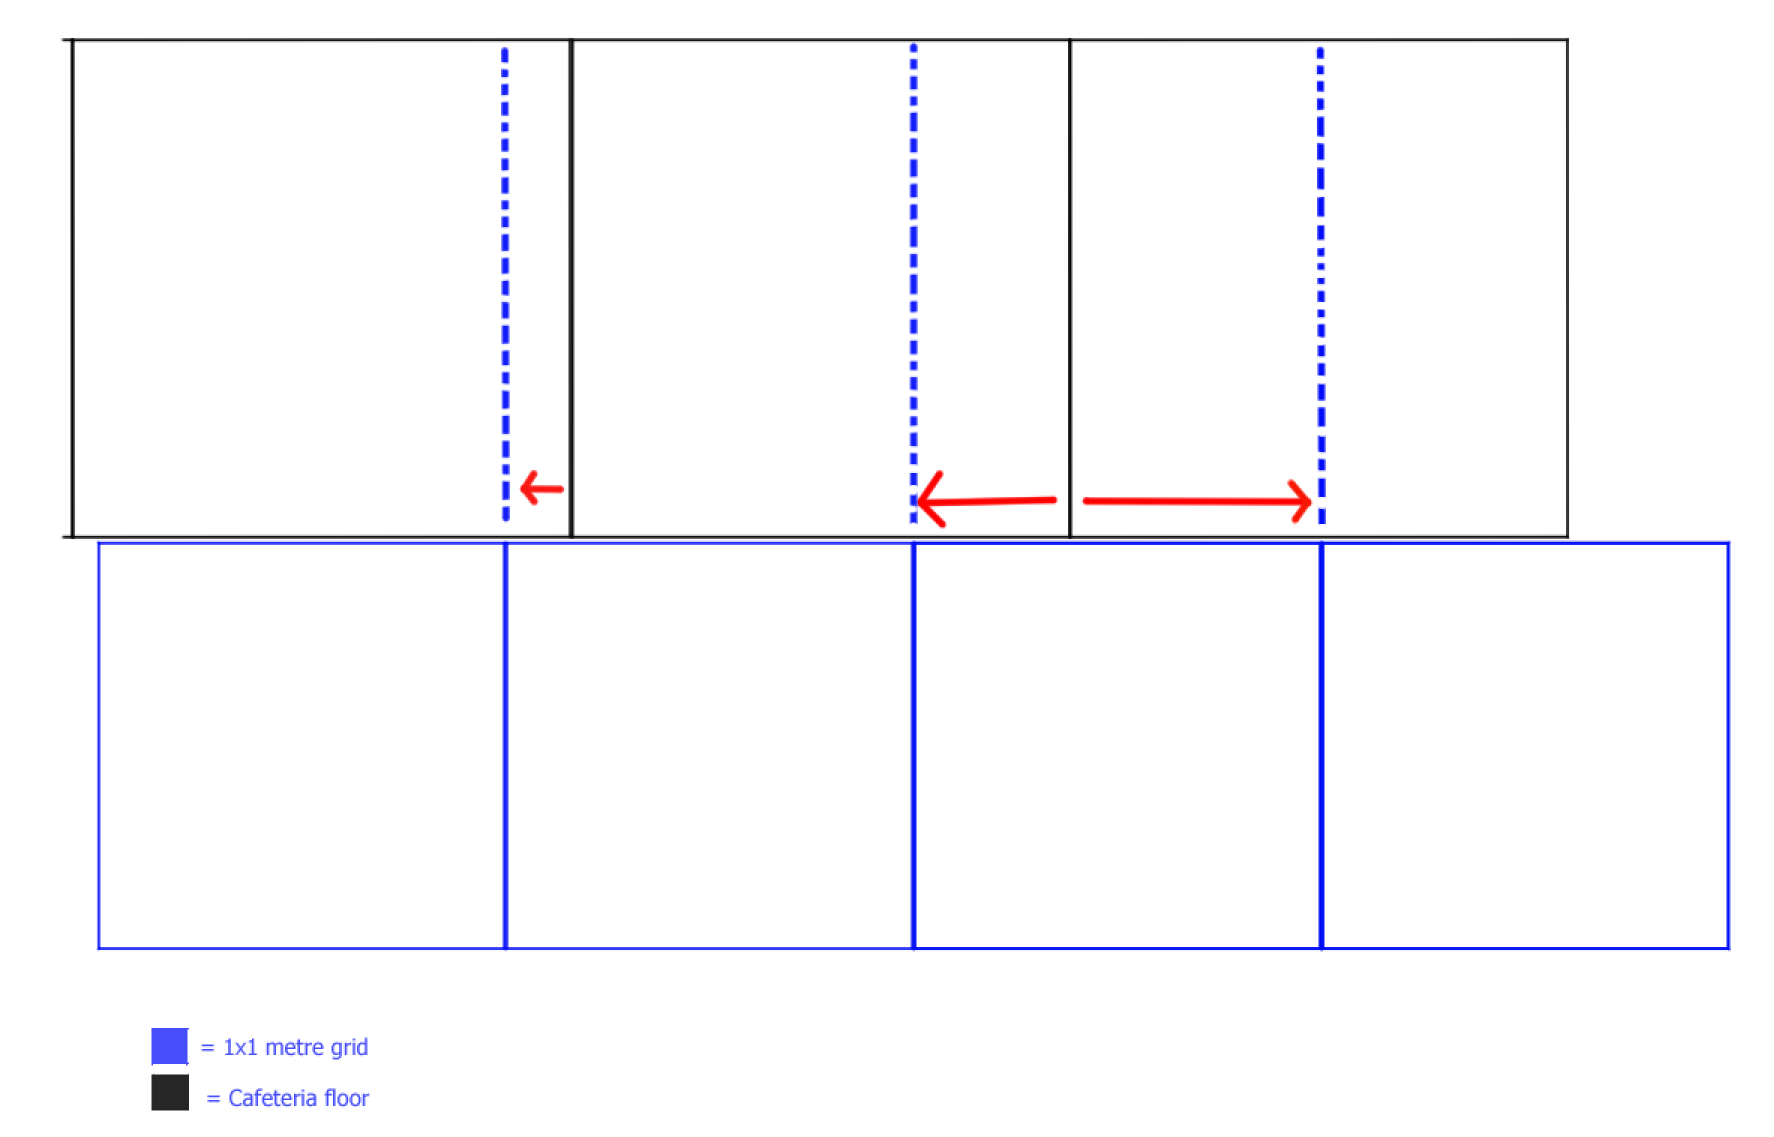
\includegraphics[width=\textwidth,height=10cm]{meth1.png}
		\caption{An overview of the research methodology. It divides the experiment into four main parts. (1) Identification of Environmental Factors, (2) Extraction of Environmental Factors, (3) Training of Fingerprint Matching Models, (4) Results and Evaluation}
		\label{fig:graph_step}
	\end{figure*}
	
	\section{Introduction}
	Indoor Positioning Systems (IPS) aim to help users navigate effectively inside of buildings or enclosed areas. This type of navigation proves difficult to create when using common methods for navigation. The most widely used system for navigation is the Global Navigation Satellite System (GNSS) which uses a combination of satellites and ground control stations that aim to calculate ground positions by trilateration. The most well-known GNSS is called the Global Positioning System (GPS). The usage of GPS comes with many caveats as the accuracy of the GPS diminishes when it is used indoors due to the fact that most buildings are built from dense materials like concrete and various metals, which the low power signal from the satellite can not penetrate. The usage of GPS often results in scattering, shadowing, blind spots and signal attenuation, which noticeably affects the accuracy\cite{bgp1}. That is why there have been various methods created for IPS to address the shortcomings of GNSS as well as provide accurate navigation in areas that may not be able to use GNSS
	
	There have been many methods developed for the usage of IPS. One of the most well-known and commonly used methods is trilateration. Trilateration works by measuring signal strength in relation to the distance from the transmitter via Received Signal Strength Indicator (RSSI) fingerprinting \cite{bg2}. The fingerprinting technique consists of two phases. An initial offline phase, and the following online phase. In the offline phase, radio maps are created by collecting RSSI data. The data is then passed onto the online phase where end devices calculate their position based on the coordinates assigned to each RSSI-emitting device, such as Bluetooth Low Energy~(BLE) devices. These BLE devices are often used for RSSI fingerprinting due to its low power consumption and ease of deployment. A mobile device can then be used to track a user's location by triangulating the user's device using the distance between the mobile device and the different BLEs. This is a good method as most RSSI signatures are distinct; however, there are shortcomings with this method. An example of a shortcoming is that RSSI is affected by environmental noise, which can cause errors in location estimation\cite{bgp2}. Another shortcoming is that some buildings may be unsuitable for BLEs and BLEs require precision placement to be effective.
	
	The usage of Machine Learning in conjunction with IPS has been shown to be effective to improve the performance of IPS. For example, a work by Gidey et al. \cite{bgp3} uses online heterogeneous transfer learning to improve the accuracy by combining data from different domains. By using Machine Learning algorithms such as Support vector Machines (SVM), Decision Trees, k-Nearest Neighbor (kNN), Random Forests, and Neural Networks (NN) it may be possible to remedy the shortcomings of IPS systems by treating it as a classification problem. This makes the positioning precision be within a range, so while it may not be able to provide a user's exact location, it can give a relatively reliable estimate on the user's area.
	
	In our previous work, we implemented an IPS using a large grid size (16.75×15m) to reduce the number of classification labels, making the problem more manageable within time constraints. While this approach provided a functional implementation, it left several questions unanswered. Specifically, we sought to determine how the number of data points influences IPS performance, whether a reliable IPS can be implemented with a limited number of BSSID to control feature space complexity, and how small a grid size can be while still maintaining reasonable positioning accuracy.
	Building on this prior work, this paper further explores the use of classification-based IPS by refining our approach to ground truth reliability in experimental settings. We evaluate the effects of feature filtering on model complexity, discuss the trade-offs between grid size and precision, and analyze the advantages and limitations of our implementation. To better quantify accuracy, we introduce two new evaluation metrics: Average Grid from Target (AGT) and Average Distance from Target (ADT). Through this study, we provide deeper insights into the design considerations for IPS, offering practical takeaways for improving indoor positioning accuracy.
	

	
	\section{Literature Review}
	IPS have been extensively studied, with a range of techniques developed to address the challenge of accurate localization within indoor environment. Traditional methods of IPS like Wi-Fi RSSI fingerprinting have been enhanced through the use of various ML algorithms, for example, k-Nearest Neighbor (kNN) \cite{LRE1}, \cite{LRE2}, \cite{LRE6}, Random Forest (RF) \cite{LRE1}, \cite{LRE6}, \cite{LRE5}, Support Vector Machine (SVM) \cite{LRE1}, \cite{LRE2}, \cite{LRE6} and Multi-Layer Perceptron (MLP) \cite{LRE1}, \cite{LRE2}. Because positioning can be treated as a classification problem,  ML algorithms based on statistics and regression are well-suited for this task. With this in mind, the improvement of data collection is essential, as the quality of RSSI data points significantly impact on IPS accuracy. This could be done by training datasets with readings from different devices and collected at different times of the day, as noted in \cite{LRE3}. Several studies have proposed methods to refine dataset quality to better train fingerprinting algorithms used in positioning systems, such as combining Human Activity Recognition (HAR) using sensors with fingerprint collection \cite{LRE4} and the development of coordination-based Android applications \cite{LRE7}. These efforts have contributed modest improvements to IPS performance and created chances to develop IPS even more with additional data points. 
	
	Deep learning approaches, such as Graph Neural Networks (GNNs) \cite{LRE2} and Convolutional Neural Networks (CNNs) \cite{LRE4}, have demonstrated superior performance over traditional ML algorithms when a sufficient number of data points are available. Despite existing work, key environmental variables, such as the resolution of fingerprint grids and the spatial distribution of reference points, have not been comprehensively investigated. In this paper, we emphasize the critical role of these factors in IPS and aim to systematically analyze and identify the most effective configurations for multi-floor environments. Our objective is to enhance the accuracy, reliability, and overall performance of IPS by considering various influencing parameters and optimizing system design accordingly
	
	
	
	\section{Research Methodology}
	This paper adopts a systematic and empirical research methodology with the aim of identifying environmental factors that influence the IPS. This methodology is illustrated in Fig.~\ref{fig:graph_step}.
	
	The figure illustrates the research methodology used in this paper. It is structured into four parts (1) Identification of environmental factors, (2) Extraction of data that is related to the factors, (3) Training of fingerprint matching models, and~(4) Analyzing and reviewing the results. The research began by carefully investigating and identifying environmental factors that may potentially interfere with the IPS performance. This was done through researching research papers that have investigated similar things as well as analysing the area in order to find key components that were likely to cause interference. After that, we analysed the data we collected and then generated fingerprint databases. From investigating the data, we decided to create two datasets, one with different grid sizes and the other with varying numbers of points of reference. These datasets were then used to train various ML Models which ran a different algorithm, including KNN, SVM, RF, MLP, XGBoost, XGBoost-based RF (XBGRF). Grid size was selected as a key variable in our investigation as we want to determine and measure the extent to which different grid sizes affect our results as well as find the optimal gridsize. Finally the accuracy of the location prediction created by these models were analyzed and evaluated against ground truth data.
	
	
	
	\subsection{Identification of Environmental Factors}
	To begin collecting data which will be used to construct our fingerprint database, the environment must first be mapped and made into one which is suitable for data collection. For environmental mapping, we decided to tape up the floor into grids which matched with our gridded digital version of the floor plan. An example of the taping process can be viewed from Fig. \ref{fig:taping}. 
	
	This tape serves as reference points for our data collection device, a mobile phone, measuring RSSI values from nearby APs in the area. Naturally, the size and number of grids directly affects the number of collected datapoints. The larger the grid size the fewer data points are present. However; larger grid-sizes also have benefits as it may help reduce localisation errors and make it easier for the models to estimate the correct grid.
	
	
	One challenge encountered during the taping process was the varying layout across different areas. Certain sections of the floor did not feature uniform tiling, with discrepancies in elevation and angle. This issue was effectively mitigated by constructing grids based on previously mapped reference points. Although minor measurement inaccuracies may exist, these are considered negligible for the purposes of this study.
	
	While taping and collecting data points, another factor that could interfere with the IPS collection presented itself. The specific area inside the grid also affected how many RSSI values were present. For instance, collecting data in the top left corner of the grid could produce different RSSI values compared to the center of the grid. This issue could be addressed by either (1) removing the edge grids and (2) collecting fewer data points in the edge grid. However, both methods result in fewer data points being collected and have minimal impact on IPS performance. Therefore, for this study, the edge grid factor is negligible and omitted from further analysis.
	
	\begin{figure}[htbp]
		\centerline{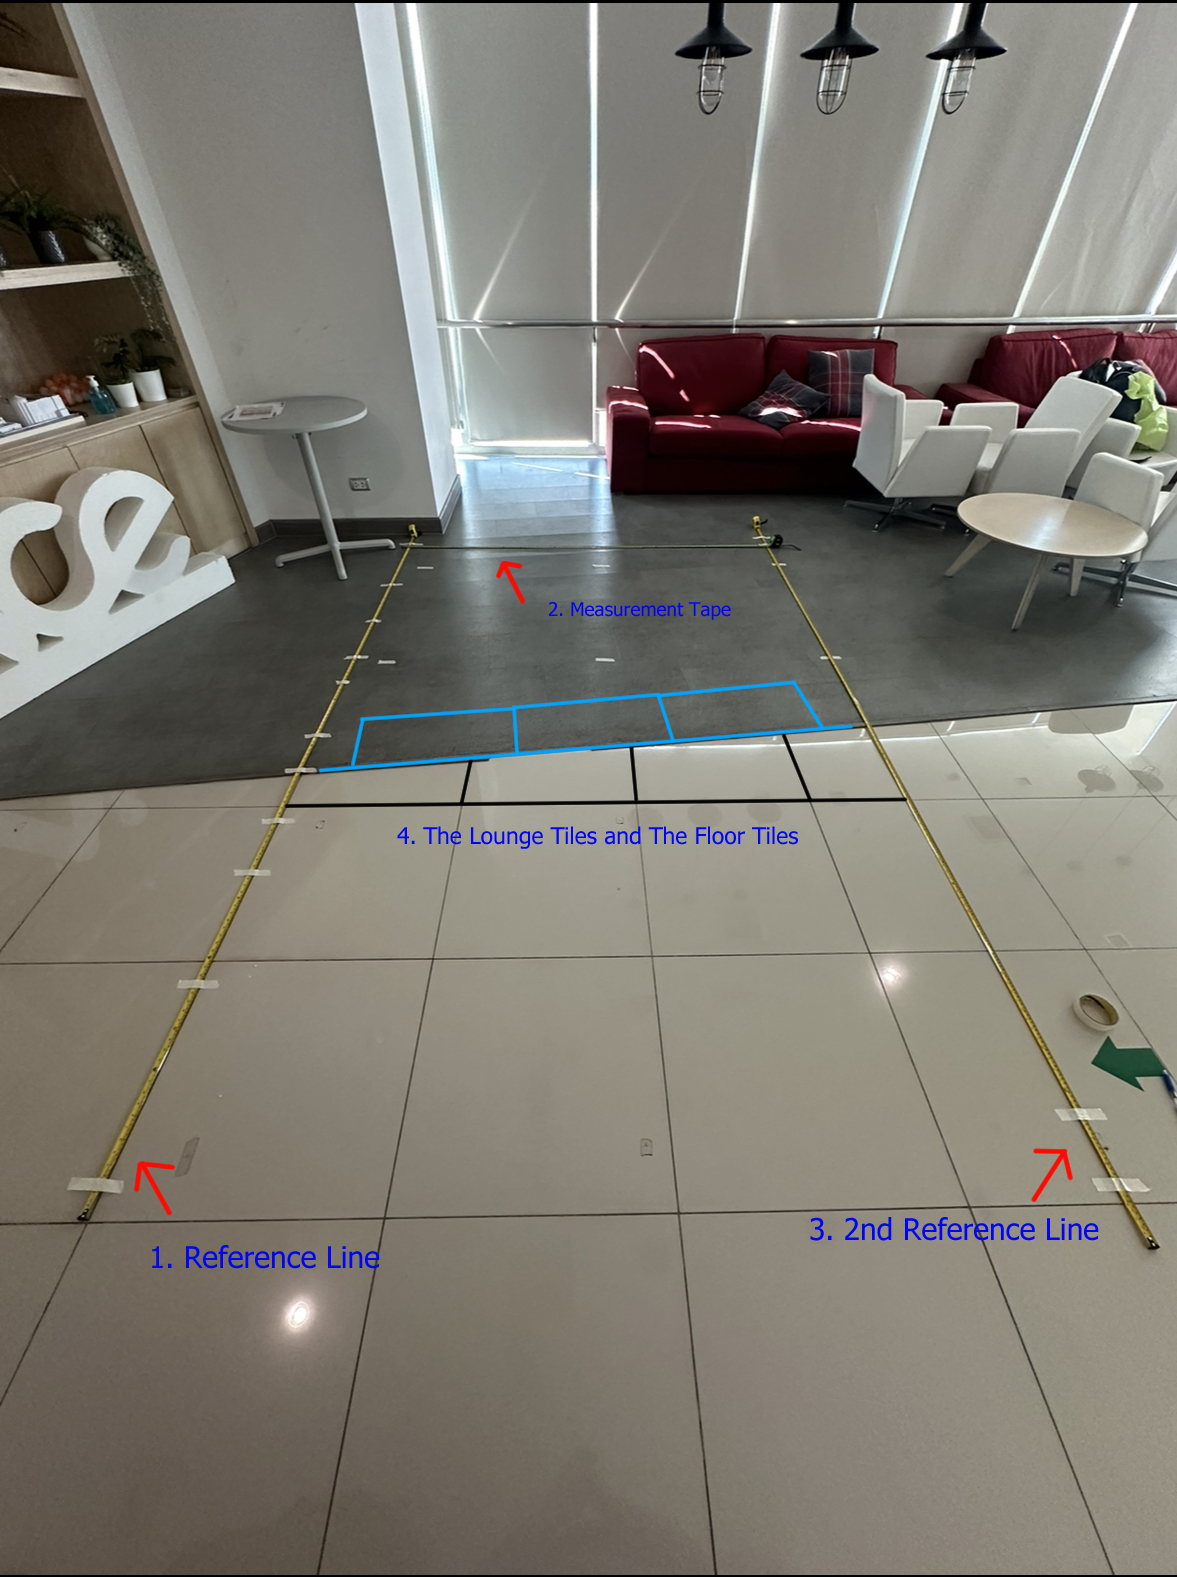
\includegraphics[scale=0.21]{meth2.jpg}}
		\caption{An example of taping that was done to create grids for data collection of RSSI values as fingerprints}
		\label{fig:taping}
	\end{figure}
	
	A similar issue arose concerning the alignment of the data structure used to assign unique labels to each grid across different floors. This challenge was particularly pronounced when experimenting with varying grid sizes, as the total area and layout of each floor differed significantly. Given the nature of this study, it was determined that the most practical approach was to treat each grid as a uniquely identifiable unit based on its grid ID. This decision was supported by the assumption that, in a classification model, sufficiently distinct features—such as differing numbers or distributions of BSSID signals observed in the same relative location on different floors—would enable the model to distinguish between grids effectively. Thus, treating each grid as uniquely distinct was not considered a limitation in this context.
	
	To validate the assumption that each grid could be treated as a distinct unit across different floors, further analysis was conducted on the collected RSSI data. During this process, it was observed that our data collection methodology initially captured all detectable access points within the network configuration, including those originating outside the intended environment. Specifically, access points from neighboring buildings were occasionally included in the dataset. Although these external access points typically exhibit low signal strength, their presence could still influence the training of fingerprint-based localization models, introducing effects similar to those found in zero-inflated spatial data.
	
	To mitigate this issue and prevent the feature space from becoming overly complex, we applied a filtering criterion that retained only access points associated with the specific campus network. This ensured that the resulting dataset focused on relevant features while maintaining consistency across grids.
	As illustrated in the heatmap in Fig. \ref{fig:heatmap008} (included here for supplementary context), some access points still exhibit non-zero RSSI values despite being on the lower end of the signal strength spectrum. These low-strength signals, represented by the darker regions on the map, may pose challenges for machine learning models during training by introducing noise and increasing the risk of underfitting.
	Through this analysis, two key factors emerged as the most influential in determining IPS performance. The first is grid size, which involves a trade-off between localization precision and the practicality of data collection. The second is the presence of low-relevance RSSI values, which—if left unfiltered—could adversely impact model performance. Taken together, these findings further support our approach of treating each grid as a unique unit, as both physical and feature-based variations across floors reinforce their distinctiveness.
	
	\begin{figure}[htbp]
		\centerline{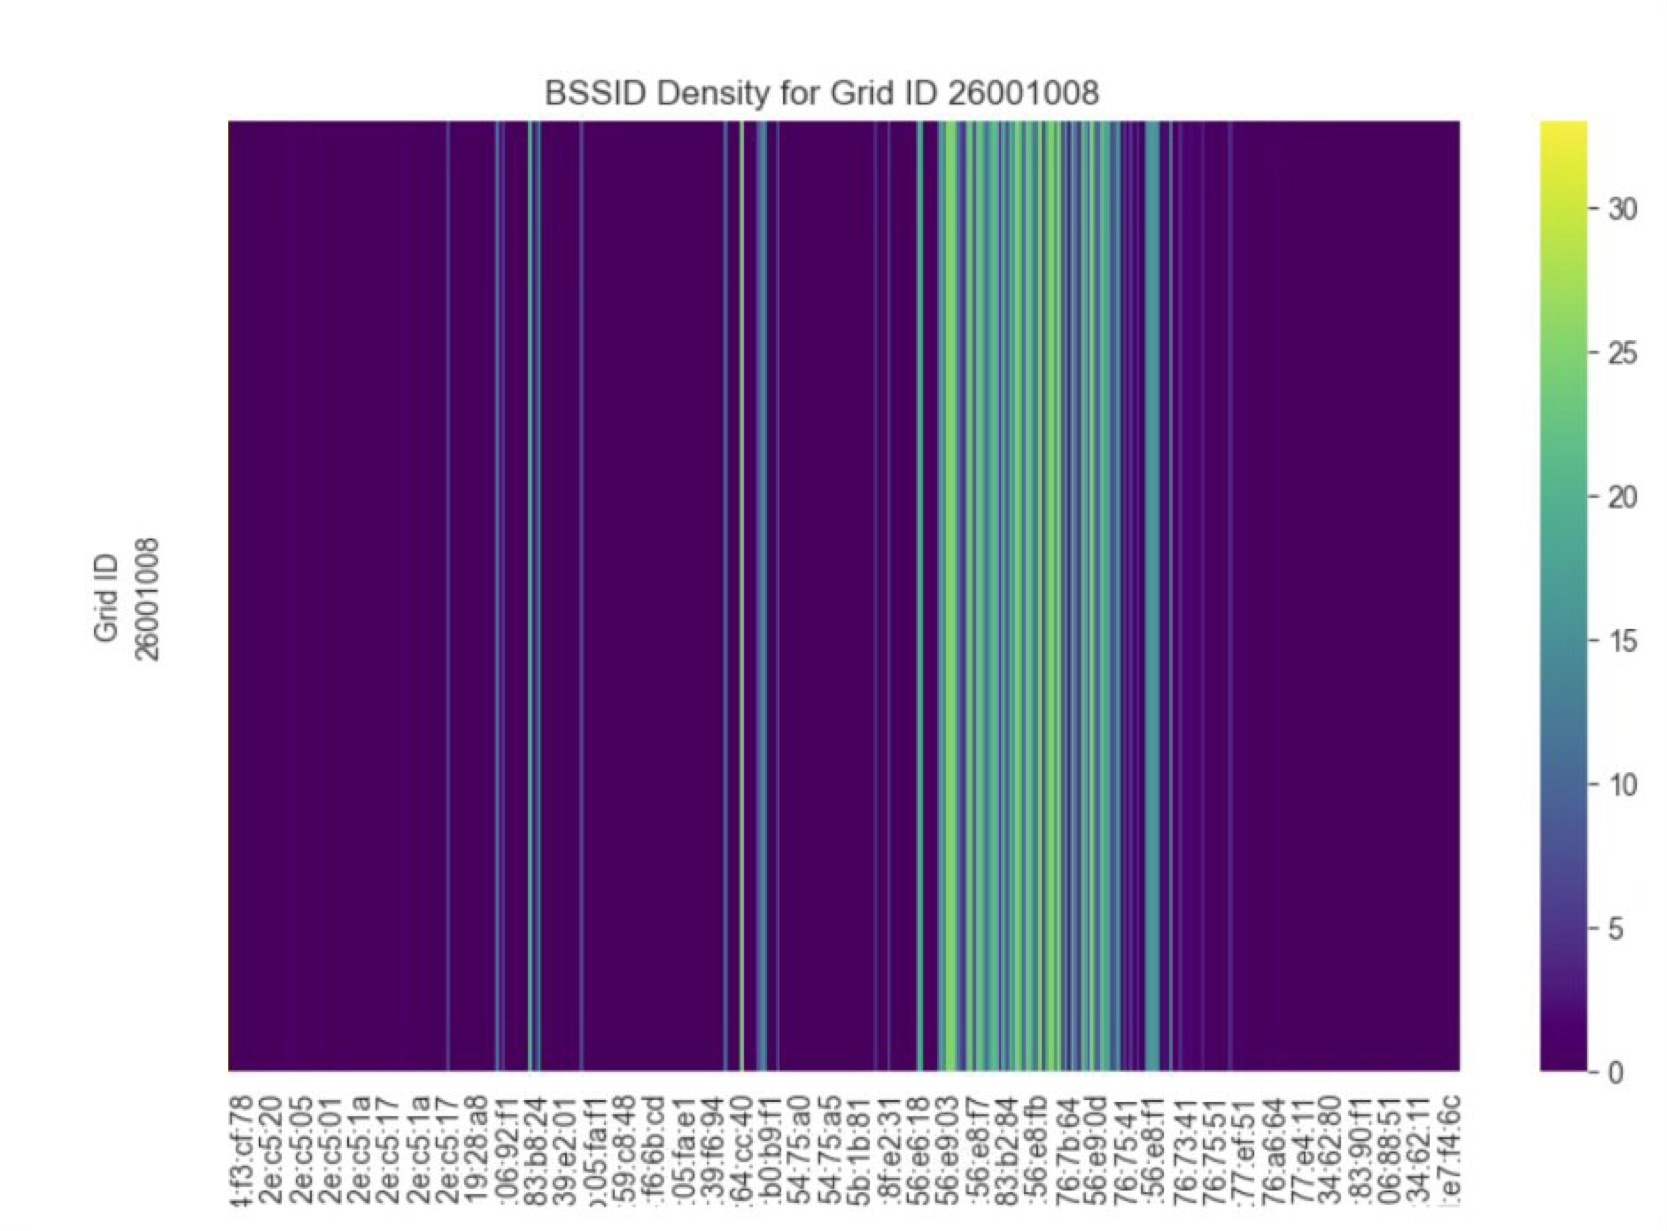
\includegraphics[scale=0.15]{meth3.jpg}}
		\caption{A heatmap that shows different access point’s RSSI values (referred to as BSSID) for a grid.}
		\label{fig:heatmap008}
	\end{figure}
	
	
	\subsection{Extraction of Environmental Factors and Datasets}
	The identification of the two factors in the previous section allows us to make adjustments to find the optimal setting for these values to maximize the IPS performance.
	
	\paragraph{Grid Size Requirements and Datasets} Grid size influences IPS performance. Its size influences the accuracy of the algorithm, as well as the ease of data collection. The following study [4] ran a model with grid sizes of 16.75 x 15m and reported high IPS performance in terms of AGT, as the larger the area, the more likely you’ll estimate the correct grid. The trade off was that the ADT was significantly lower, as there was a deviation from the actual point. This suggests that by minimising the grid size, we can achieve a higher precision. However the lower the precision, the harder the data collection process. 
	If we were to collect data for varying grid sizes with the taping method it would be extremely difficult as taping and re-taping the area multiple times is not feasible for a small team. Instead, we have formulated an approach through the usage of RSSI value interpolation. This allows us to form larger grid sizes from combining smaller grids. We use the data collected from small grids i.e. (1m x 1m) and then aggregate them to construct larger grids by interpolating RSSI values from the combined smaller grids.
	
	By collecting 5 datapoints in a grid, the top left, top right, bottom left, bottom right and centre we can interpolate these RSSI values into a combined grid by averaging the values from the individual grids.
	
	For example, when creating a 2m x 2m grid, we do this by determining a value where the sum of distances between the RSSI values of the centres are all 0 in all four grids and then interpolating them. This method works as our grid sizes were 1m x 1m grids.
	
	\begin{figure}[htbp]
		\centerline{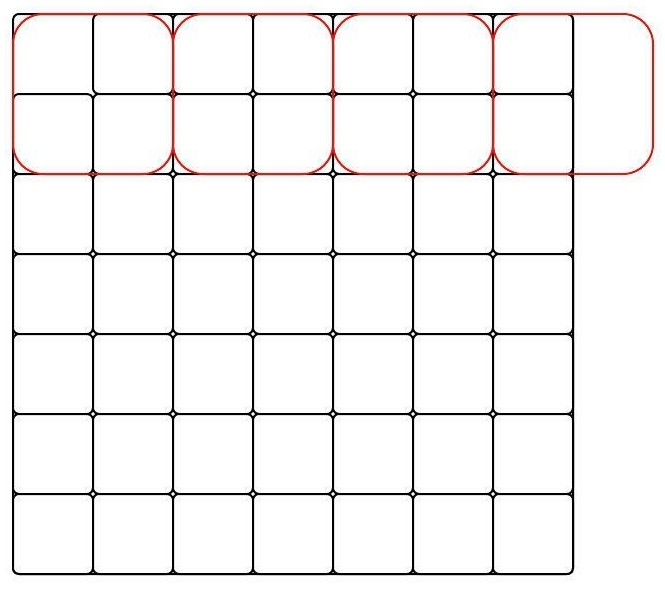
\includegraphics[scale=0.5]{image14.jpg}}
		\caption{Visualizing grid resizing}
		\label{fig:vis_grid_resize}
	\end{figure}
	
	\paragraph{Unrelated RSSI Value Filtering and Datasets} Many points exhibit low RSSI values as shown previously in fig. \ref{fig:heatmap008}. To avoid underfitting, we have chosen to omit these values from our model. However; the removal of these values does not guarantee that the model will have improved accuracy. To measure this, we have created two datasets, one with all the access points and one with the omitted RSSI values. We can then compare the results of both datasets to determine the impact that these omitted values have on the performance of our IPS system.
	
	We also considered implementing white-listing of access points within the targeted area, but we realised that this was not required as by doing so for a mult-floor model would result in our dataset exhibiting characteristics similar to an unfiltered dataset.
	
	
	\section{Result}
	\begin{table}[htbp]
		\centering
		\begin{tabular}{|c|c|c|}
			\hline
			\multicolumn{2}{|c|}{\textbf{Collected Data Points}} & \textbf{\# BSSID} \\
			\hline
			\multirow{2}{*}{\textbf{Filtering Features}} & \textbf{Non-Filtered} & 1799 \\
			\cline{2-3}
			& \textbf{Filtered}     & 378  \\
			\hline
		\end{tabular}
		\caption{Total Bssid Before and After Filtering}
		\label{tab:bssid_counts}
	\end{table}
	
	\begin{table}[htbp]
		\centering
		\begin{tabular}{|c|c|c|c|c|c|c|c|c|}
			\hline
			\makecell{\textbf{Grid}\\\textbf{Count}} & \multicolumn{8}{c|}{\textbf{Grid Size Variations}} \\
			\cline{2-9}
			& 1x1 & 3x3 & 5x5 & 7x7 & 9x9 & 11x11 & 13x13 & 15x15 \\
			\hline
			\textbf{Total Grid} & 483 & 96 & 47 & 29 & 28 & 16 & 18 & 9 \\
			\hline
		\end{tabular}
		\caption{Total unique Grid present and Used for each grid size experiment training}
		\label{tab:grid_size_variations}
	\end{table}
	
	\begin{table}[htbp]
		\centering
		\begin{tabular}{lllll}
		\cline{1-3}
		\multicolumn{1}{|l|}{}              & \multicolumn{2}{l|}{\textbf{Floor}}                          &  &  \\ \cline{1-3}
		\multicolumn{1}{|l|}{\textbf{1x1 Grid Size}} & \multicolumn{1}{l|}{1st}   & \multicolumn{1}{l|}{2nd}   &  &  \\ \cline{1-3}
		\multicolumn{1}{|l|}{\textbf{Grid Count}}    & \multicolumn{1}{l|}{309} & \multicolumn{1}{l|}{174} &  &  \\ \cline{1-3}
		&                          &                          &  & 
		\end{tabular}
		\caption{Total true unique grid}
		\label{tab:Total true unique grid} 
	\end{table}
	
	The dataset used in this study consisted of 12,640 data points collected across 1x1m\textsuperscript{2} grids distributed among the floors of our experimental setup. By filtering the available BSSID to utilize only SSID with specific identifiers, we end up with 378 unique BSSID, spanning across the 2 floors of the experiment. A rationale behind filtering WiFi signals in this experiment is to determine whether only easily known BSSID can be utilized in implementing IPS. 9019 data points were collected on 6th floor and 3621 data points were collected on 7th floor.
	
	To explore how different parameter settings impact model training, we systematically iterate through various configurations, training the model multiple times under each setting. The table below highlights the best results observed. Notably, the highest accuracy and the best AGT (Average Grid from Target) do not come from the same parameter setting.
	
	
	
	This suggests that these metrics prioritize different aspects of performance—optimizing for accuracy does not necessarily yield the best AGT and vice versa. This insight provides a key perspective as we analyze the results in more detail. Another thing of note is, according to fig. ~\ref{fig:AGT_dgrid_size}, from 7x7m grid size onwards, our best AGT measured across different model starts to plateau which could indicate diminishing returns from increasing experiment grid size.
	
	\begin{figure}[htbp]
		\centerline{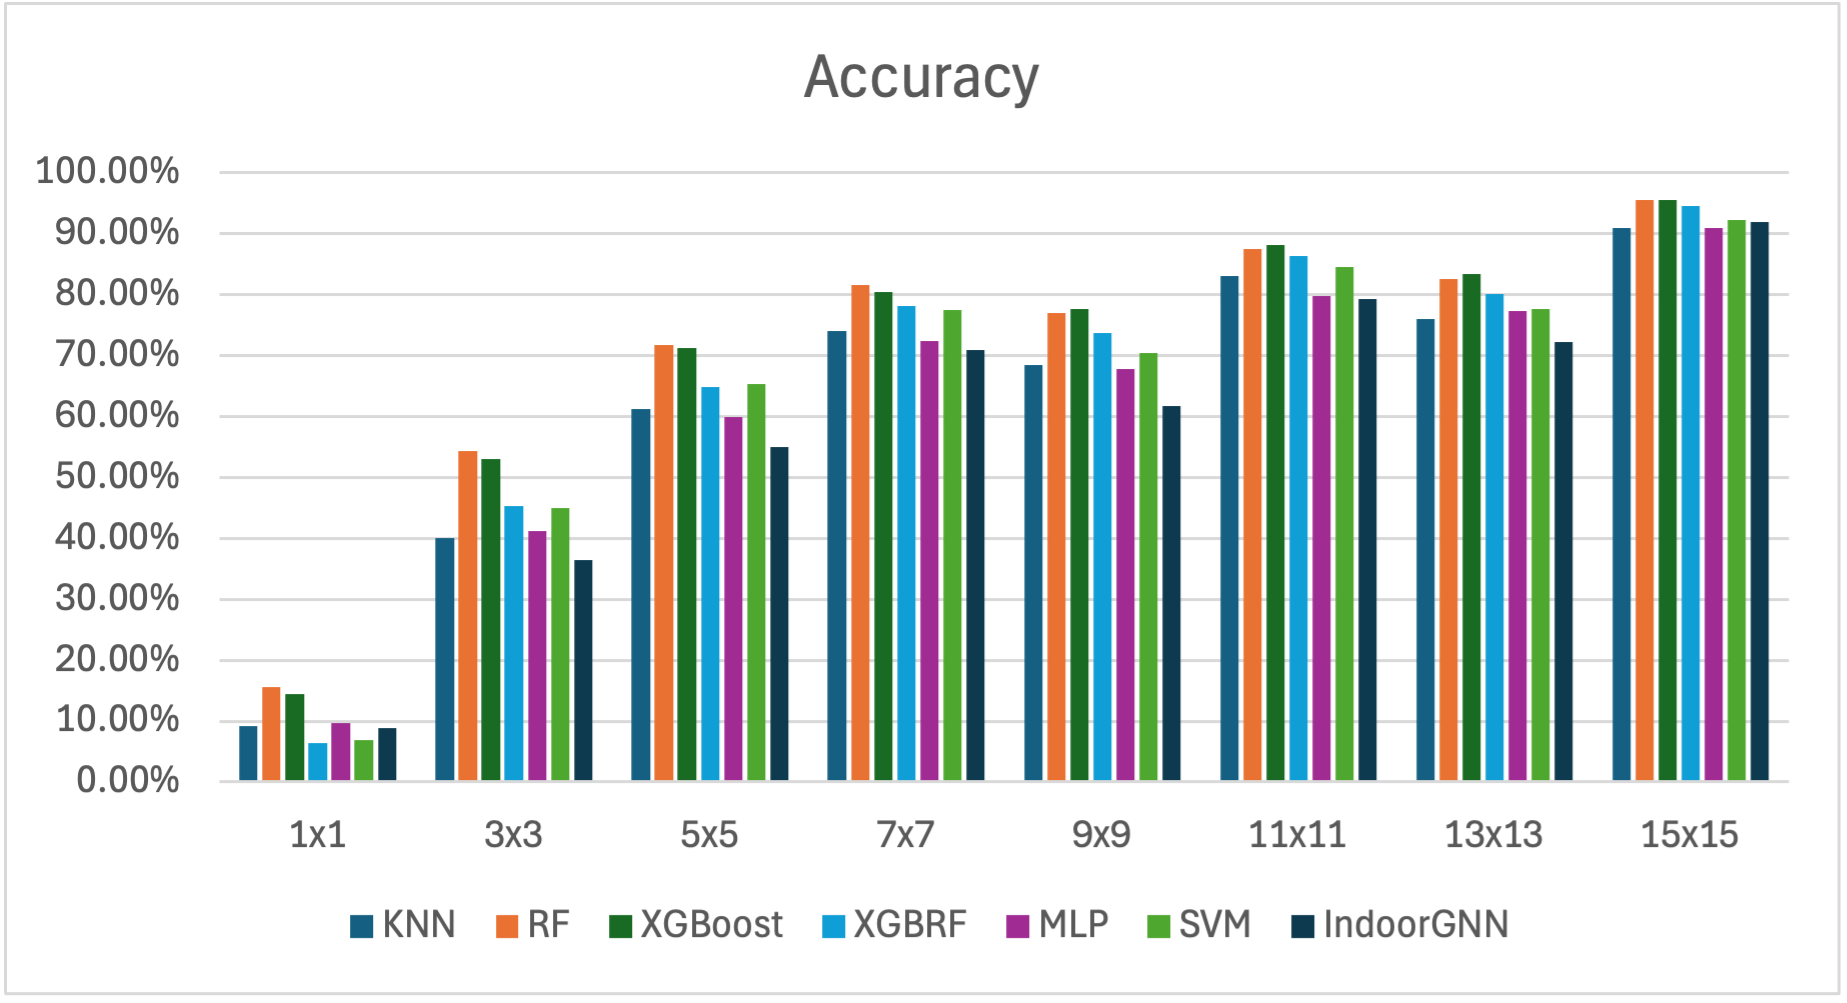
\includegraphics[scale=0.65]{image3.png}}
		\caption{Model Accuracy on Different grid size}
		\label{fig:acc_dgird_size}
	\end{figure}
	
	\begin{figure}[htbp]
		\centerline{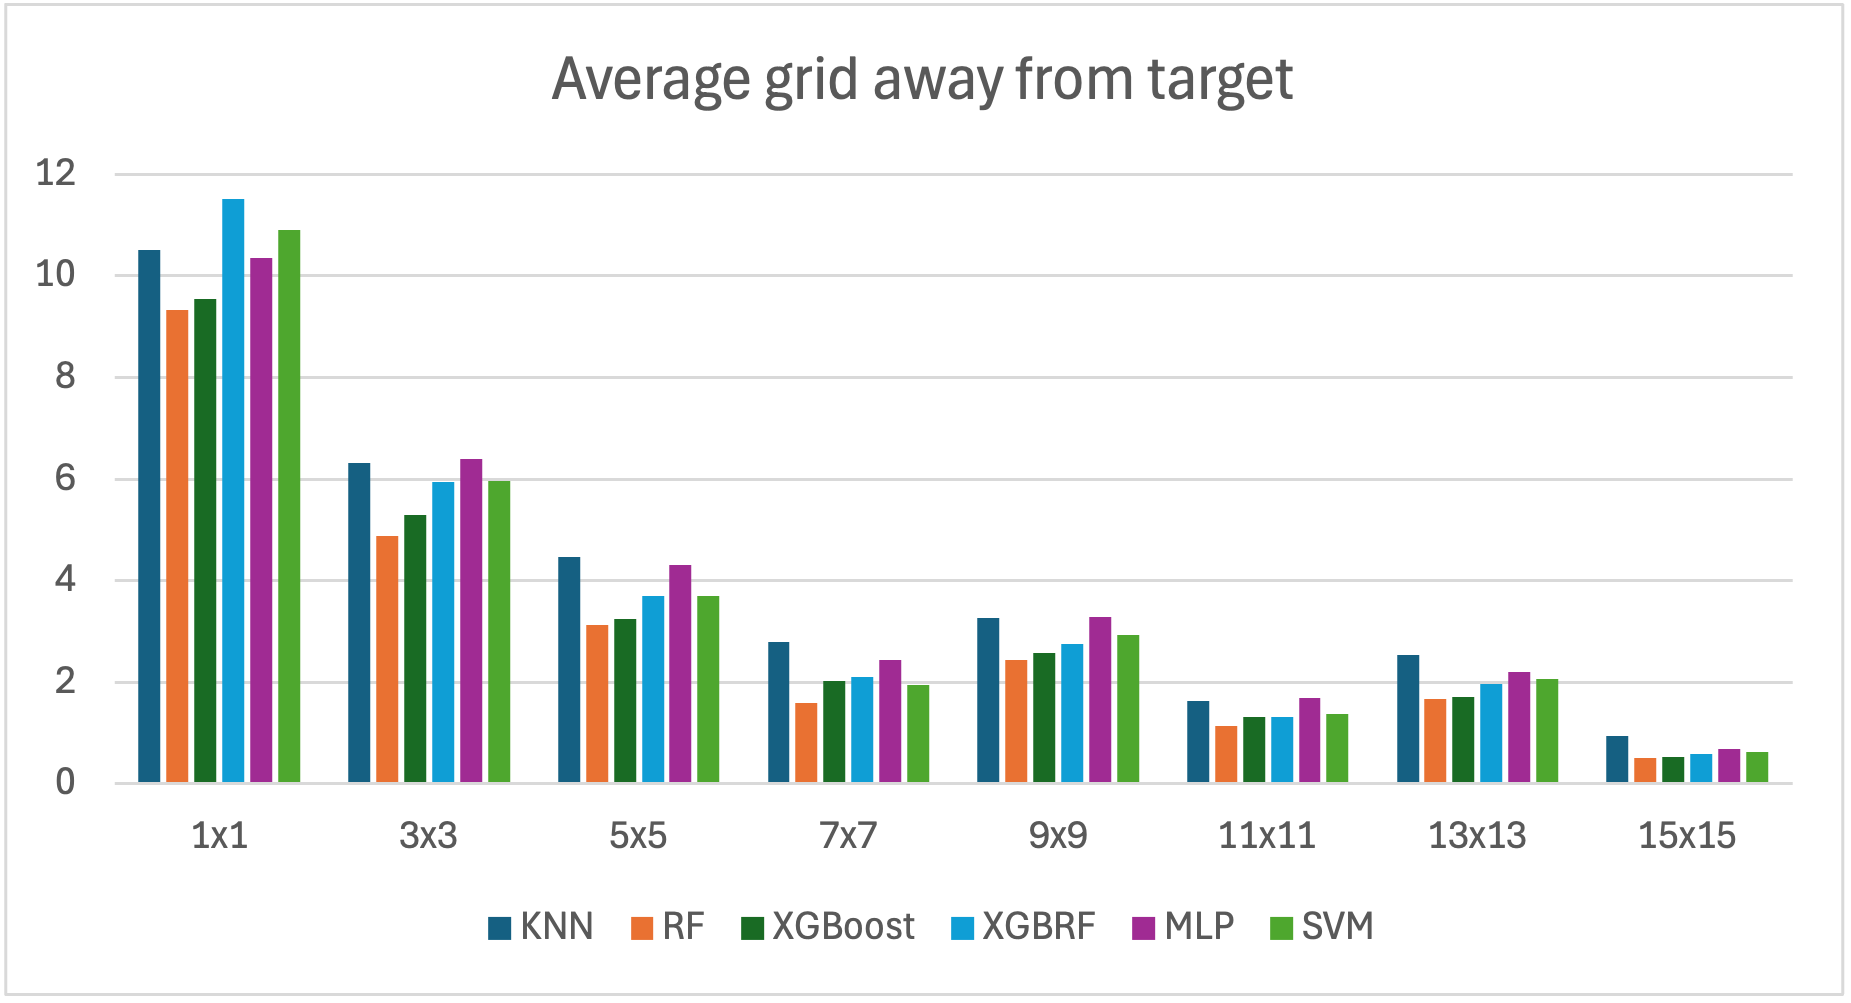
\includegraphics[scale=0.65]{image1.png}}
		\caption{Model Average grid away from Target on Different grid size}
		\label{fig:AGT_dgrid_size}
	\end{figure}
	
	\begin{comment}
	\begin{figure*}[hbt!]
		\centering
		\subfloat[Grid ID 26001008]{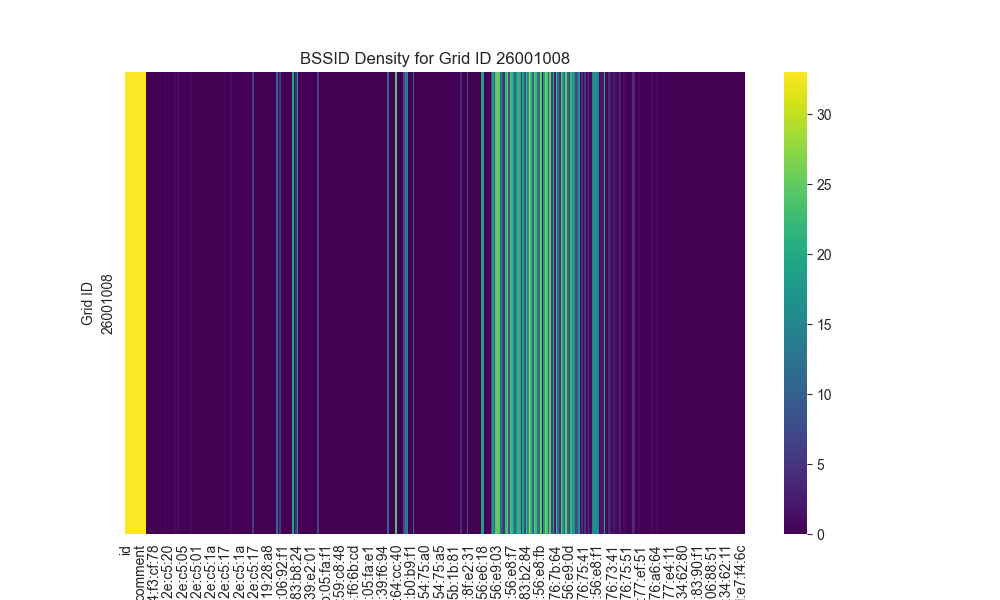
\includegraphics[width=0.45\linewidth]{heatmap_gridid_26001008.png}}
		\subfloat[Grid ID 270011123]{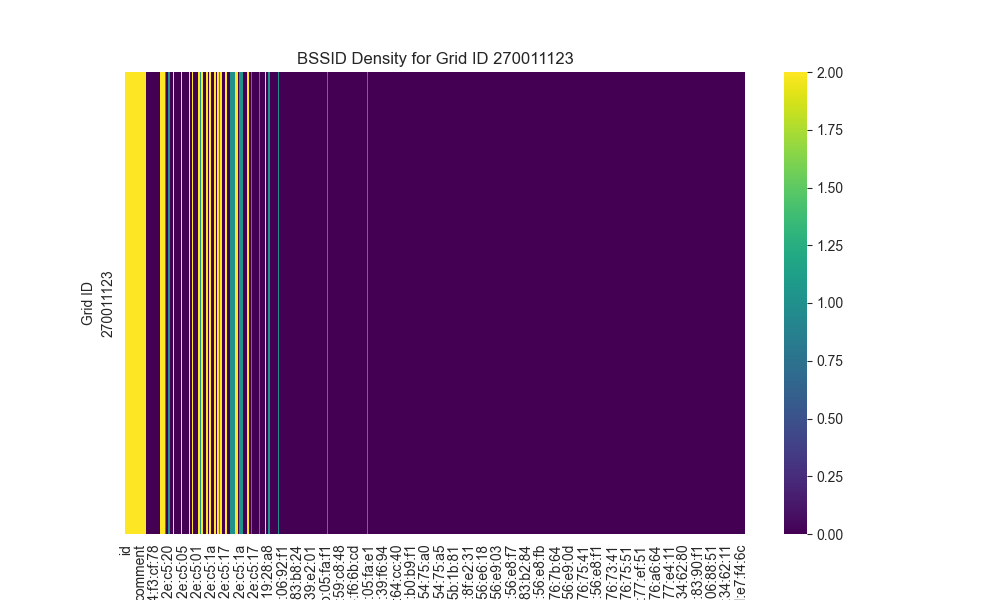
\includegraphics[width=0.45\linewidth]{heatmap_gridid_270011123.png}} \\
		
		\subfloat[Grid ID 26001407]{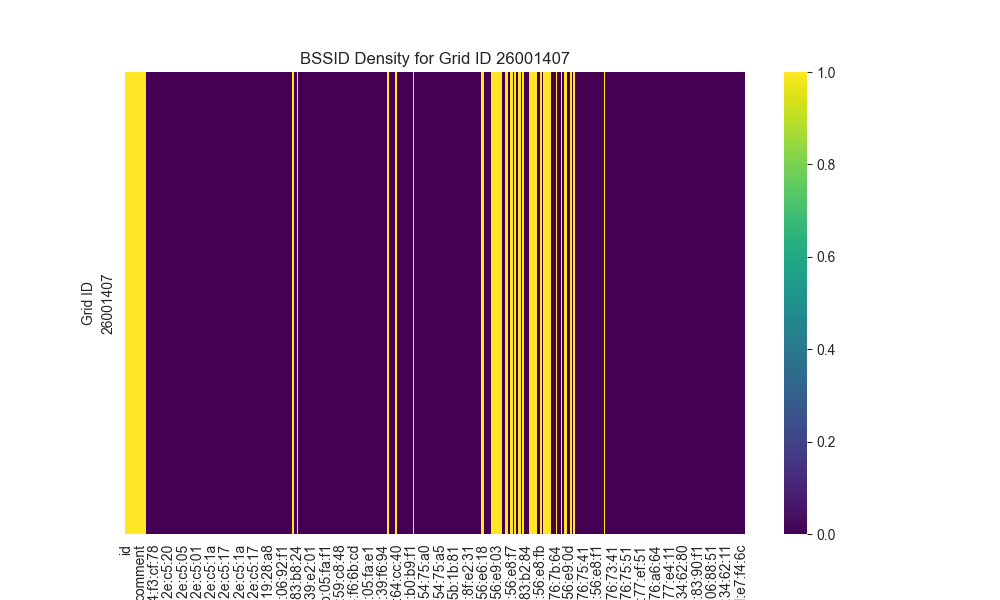
\includegraphics[width=0.45\linewidth]{heatmap_gridid_26001407.png}}
		\subfloat[Grid ID 27001786]{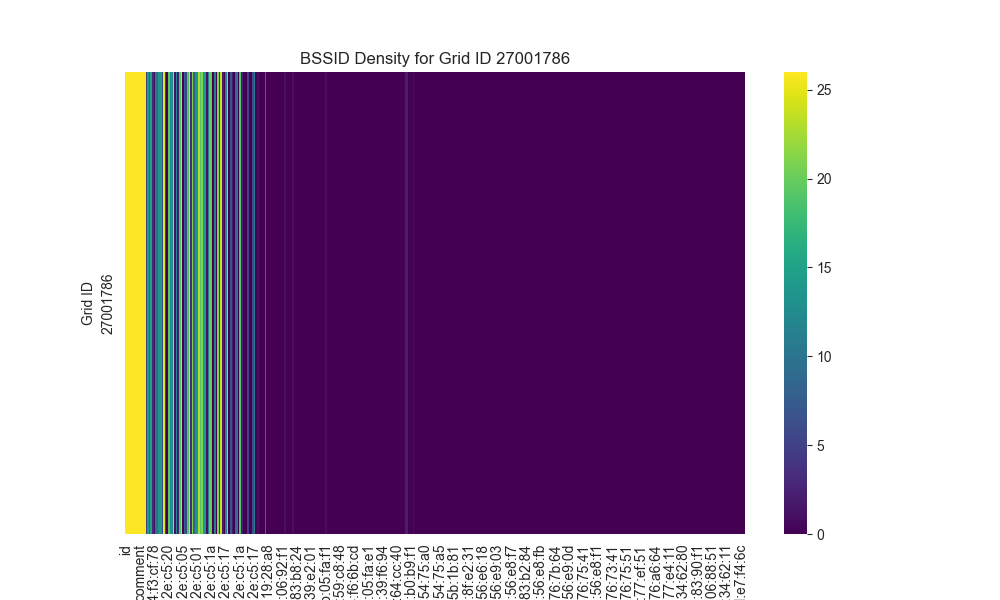
\includegraphics[width=0.45\linewidth]{heatmap_gridid_27001786.png}} \\
		
		\subfloat[Grid ID 26001811]{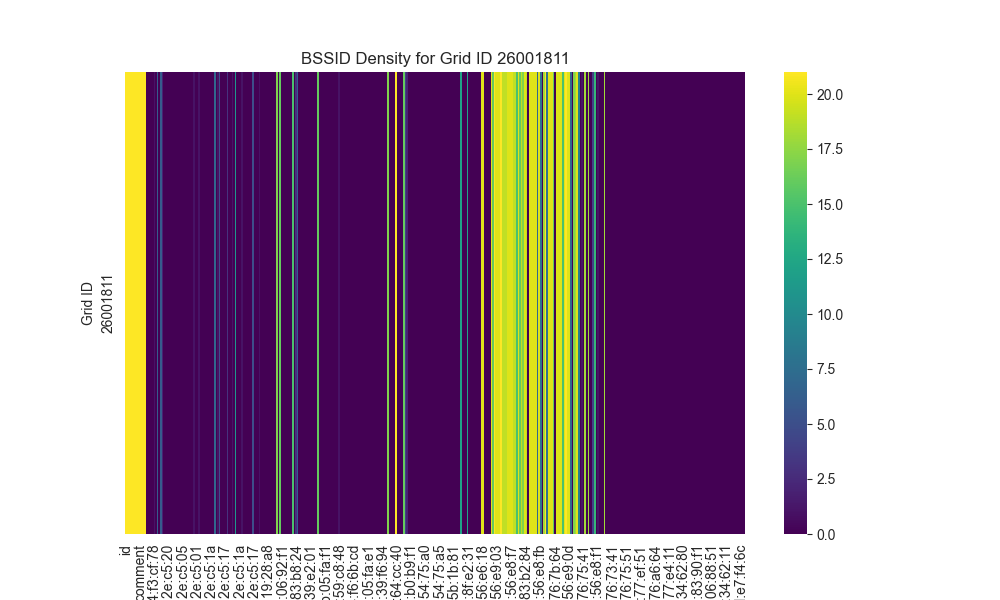
\includegraphics[width=0.45\linewidth]{heatmap_gridid_26001811.png}}
		\subfloat[Grid ID 27001918]{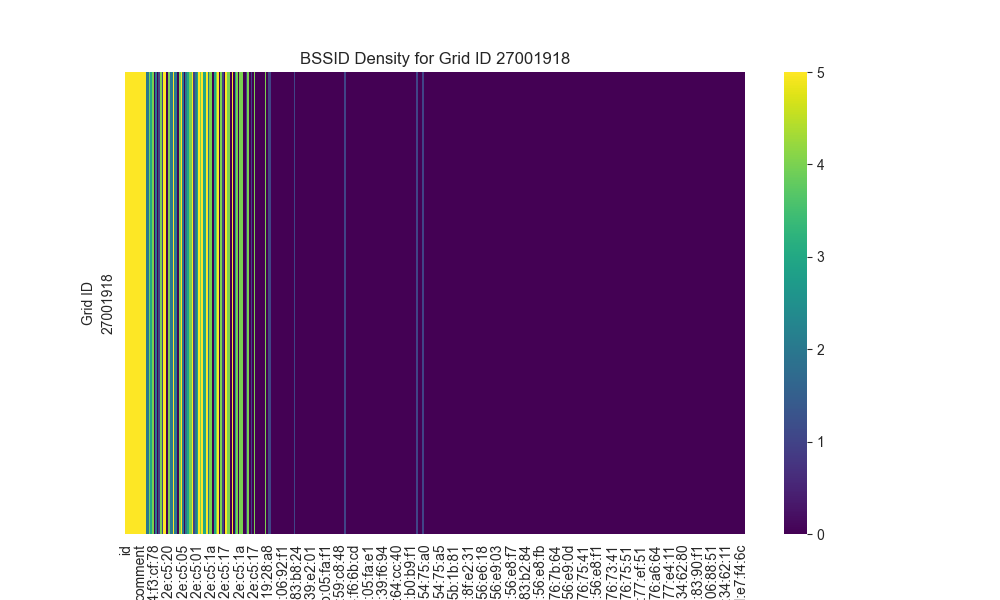
\includegraphics[width=0.45\linewidth]{heatmap_gridid_27001918.png}} \\
		
		\subfloat[Grid ID 26001888]{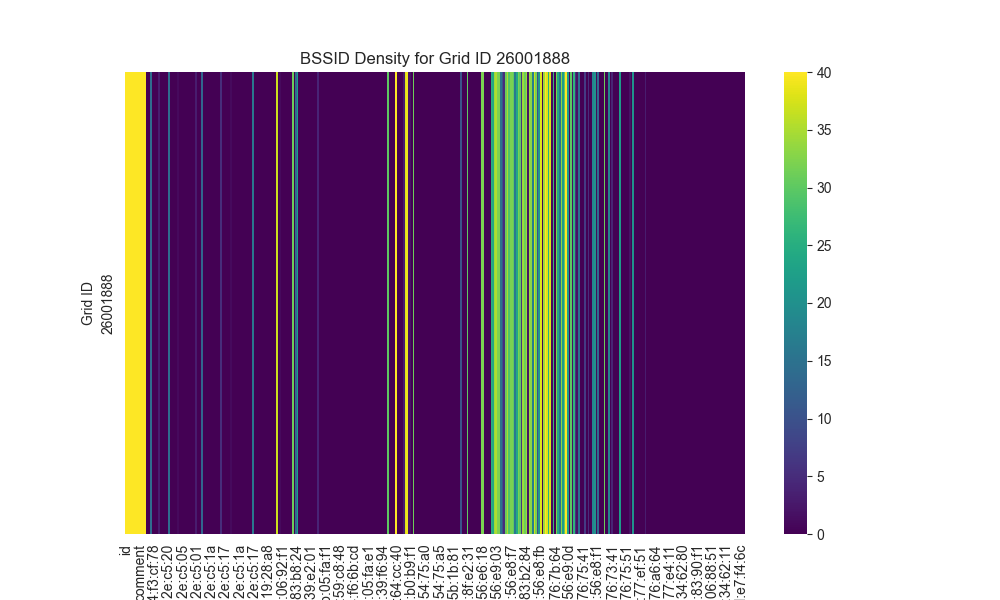
\includegraphics[width=0.45\linewidth]{heatmap_gridid_26001888.png}}
		\subfloat[Grid ID 270011051]{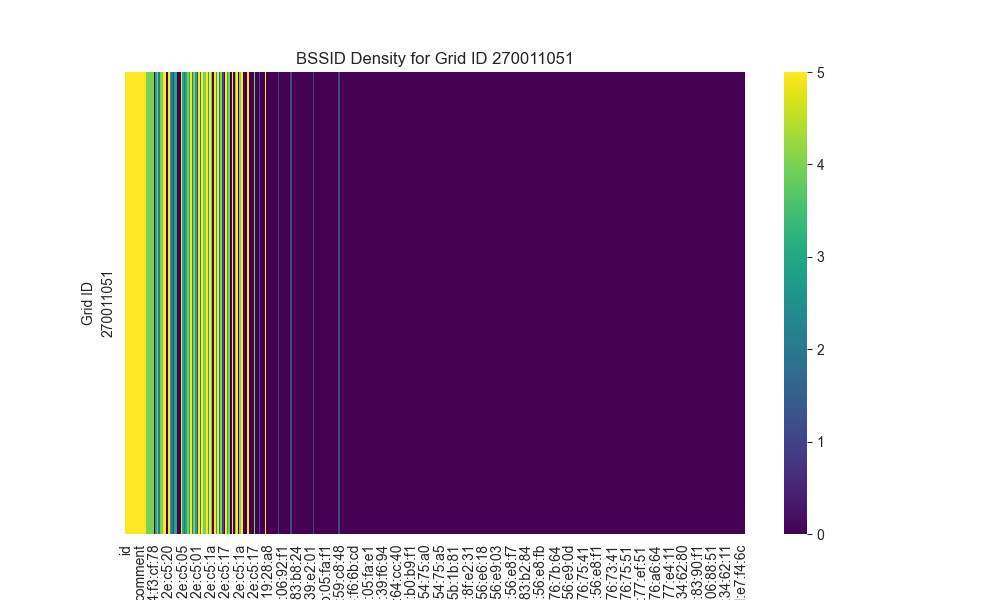
\includegraphics[width=0.45\linewidth]{heatmap_gridid_270011051.png}} \\
		
		\subfloat[Grid ID 260011369]{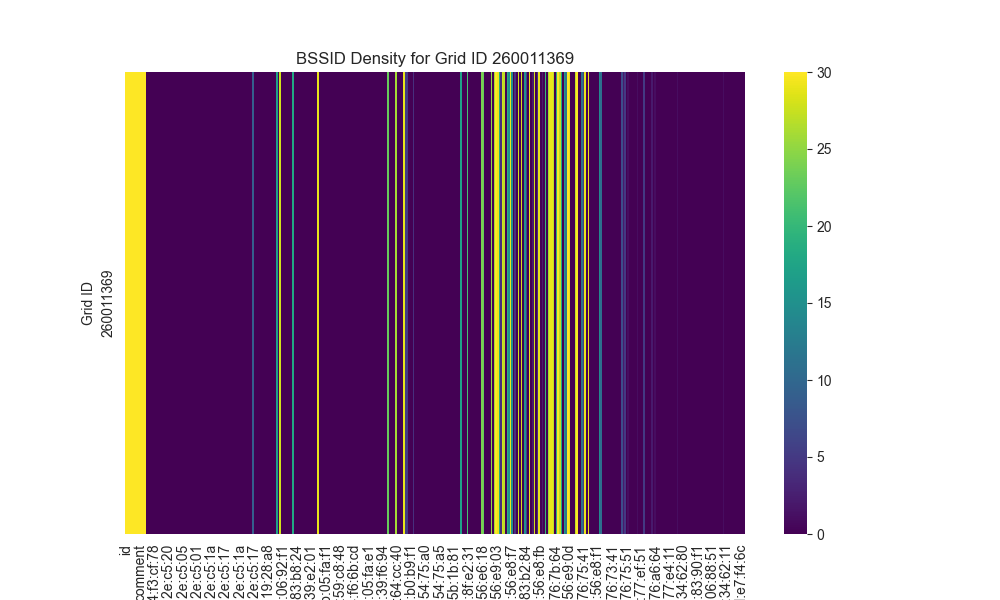
\includegraphics[width=0.45\linewidth]{heatmap_gridid_260011369.png}}
		\subfloat[Grid ID 270011105]{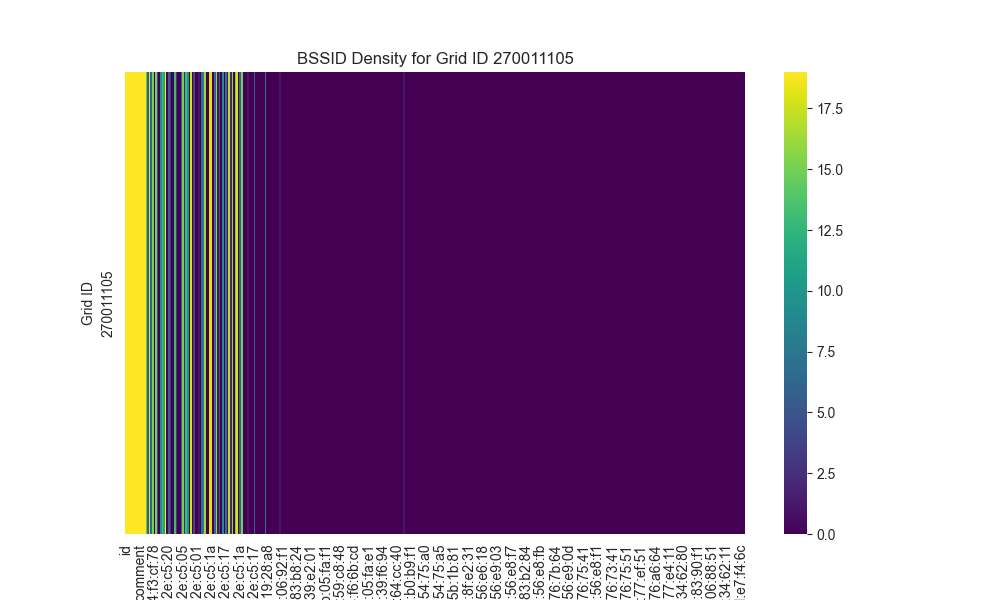
\includegraphics[width=0.45\linewidth]{heatmap_gridid_270011105.png}}
		
		\caption{BSSID Density Heatmaps for Grid IDs (26XXXX on the left, 27XXXX on the right).}
		\label{fig:gay}
	\end{figure*}
	\end{comment}
	
	\begin{figure*}[hbt!]
		\centering
		% First row
		\begin{minipage}{0.45\textwidth}
			\centering
			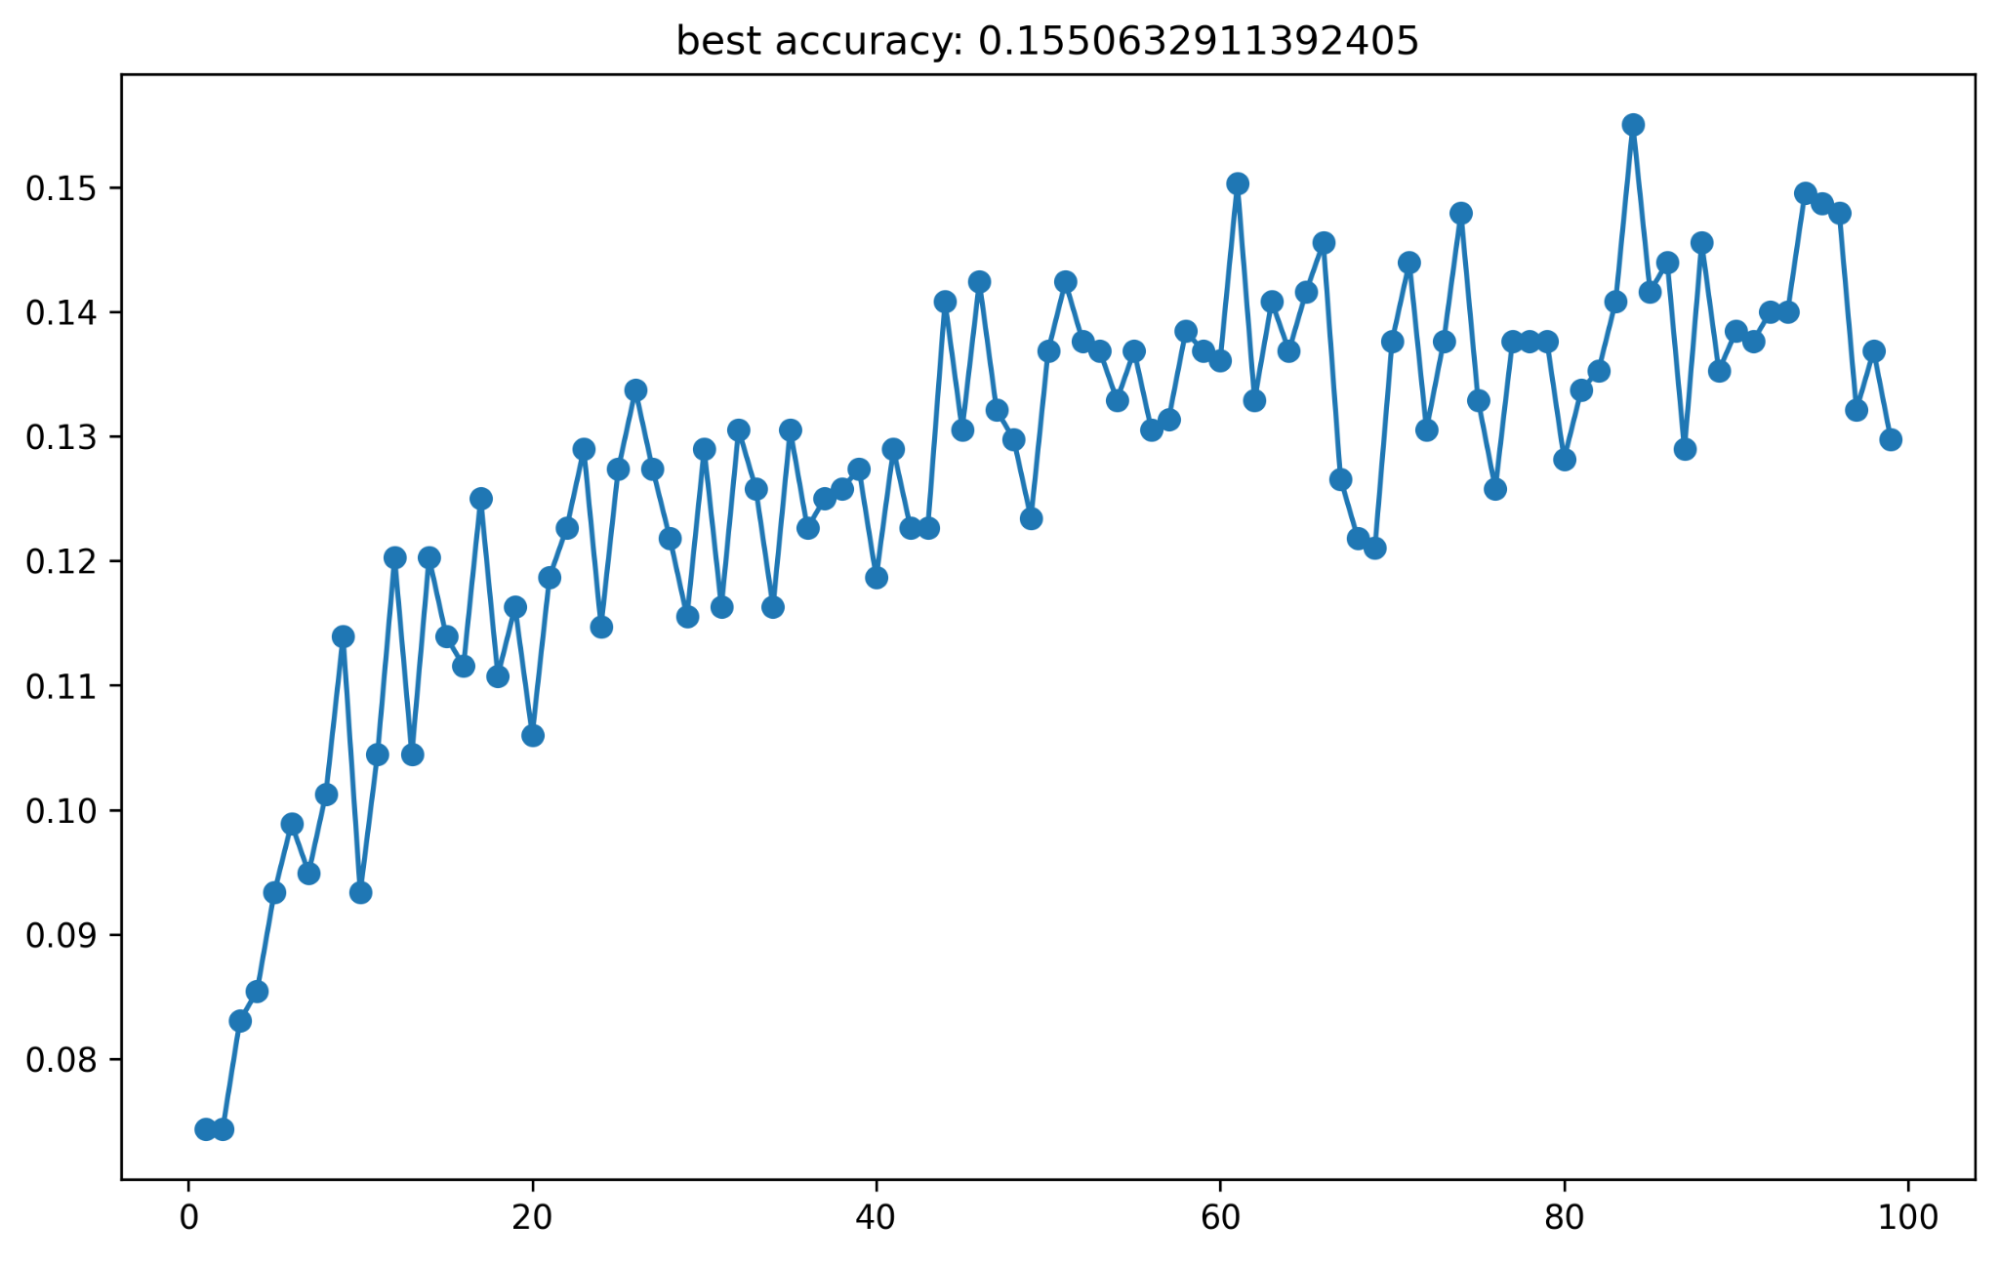
\includegraphics[width=\linewidth]{image5.png}
			\caption{RF Model accuracy with BSSID filtering (1x1)}
			\label{fig:rf_acc_filter}
		\end{minipage}
		\hfill
		\begin{minipage}{0.45\textwidth}
			\centering
			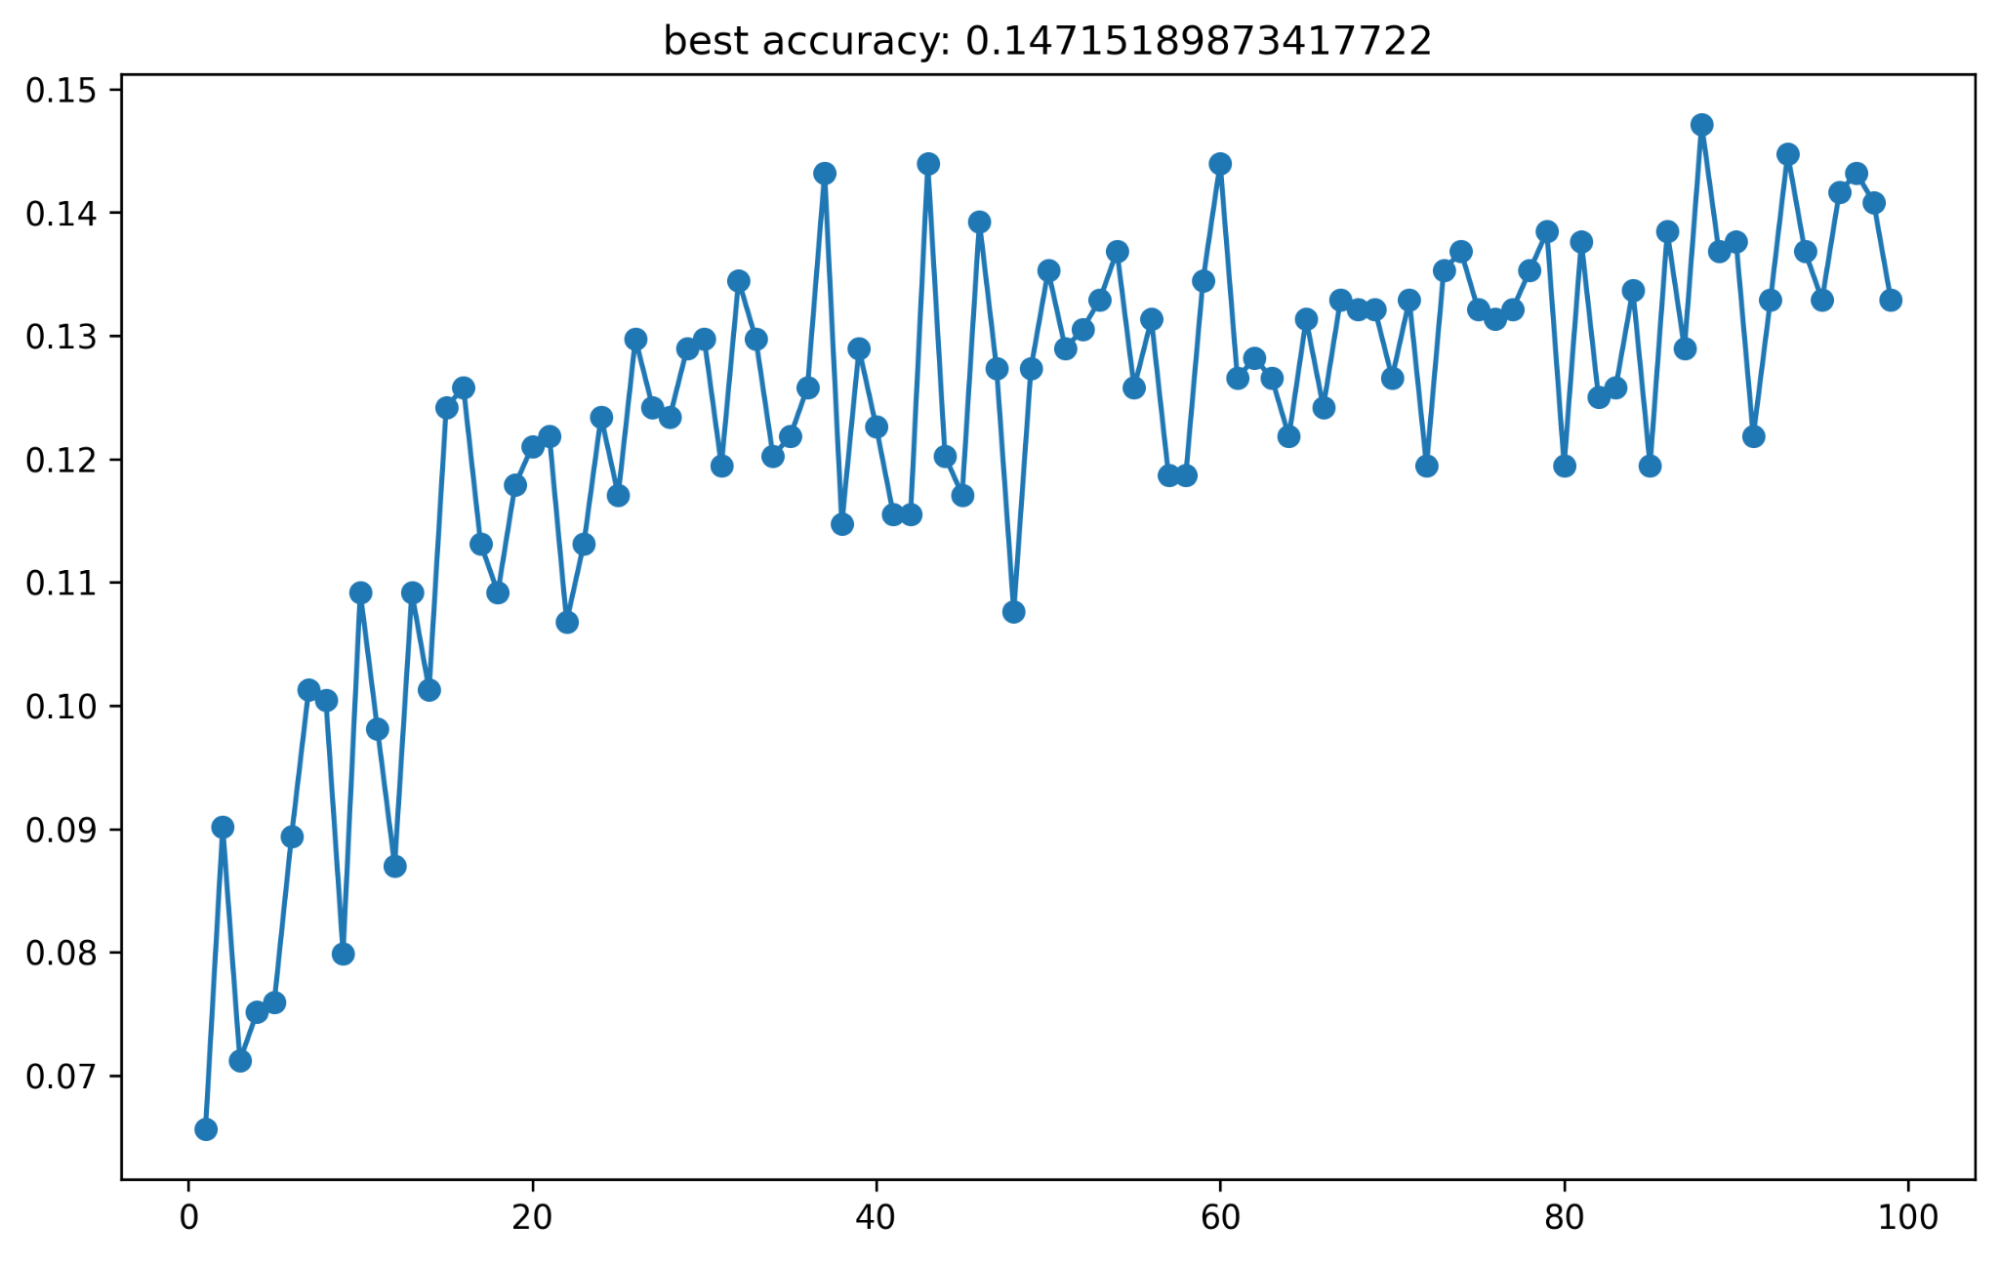
\includegraphics[width=\linewidth]{image6.png}
			\caption{RF Model accuracy without BSSID filtering (1x1)}
			\label{fig:rf_acc_nofilter}
		\end{minipage}
		
		\vspace{0.5cm} % vertical space between rows
		
		% Second row
		\begin{minipage}{0.45\textwidth}
			\centering
			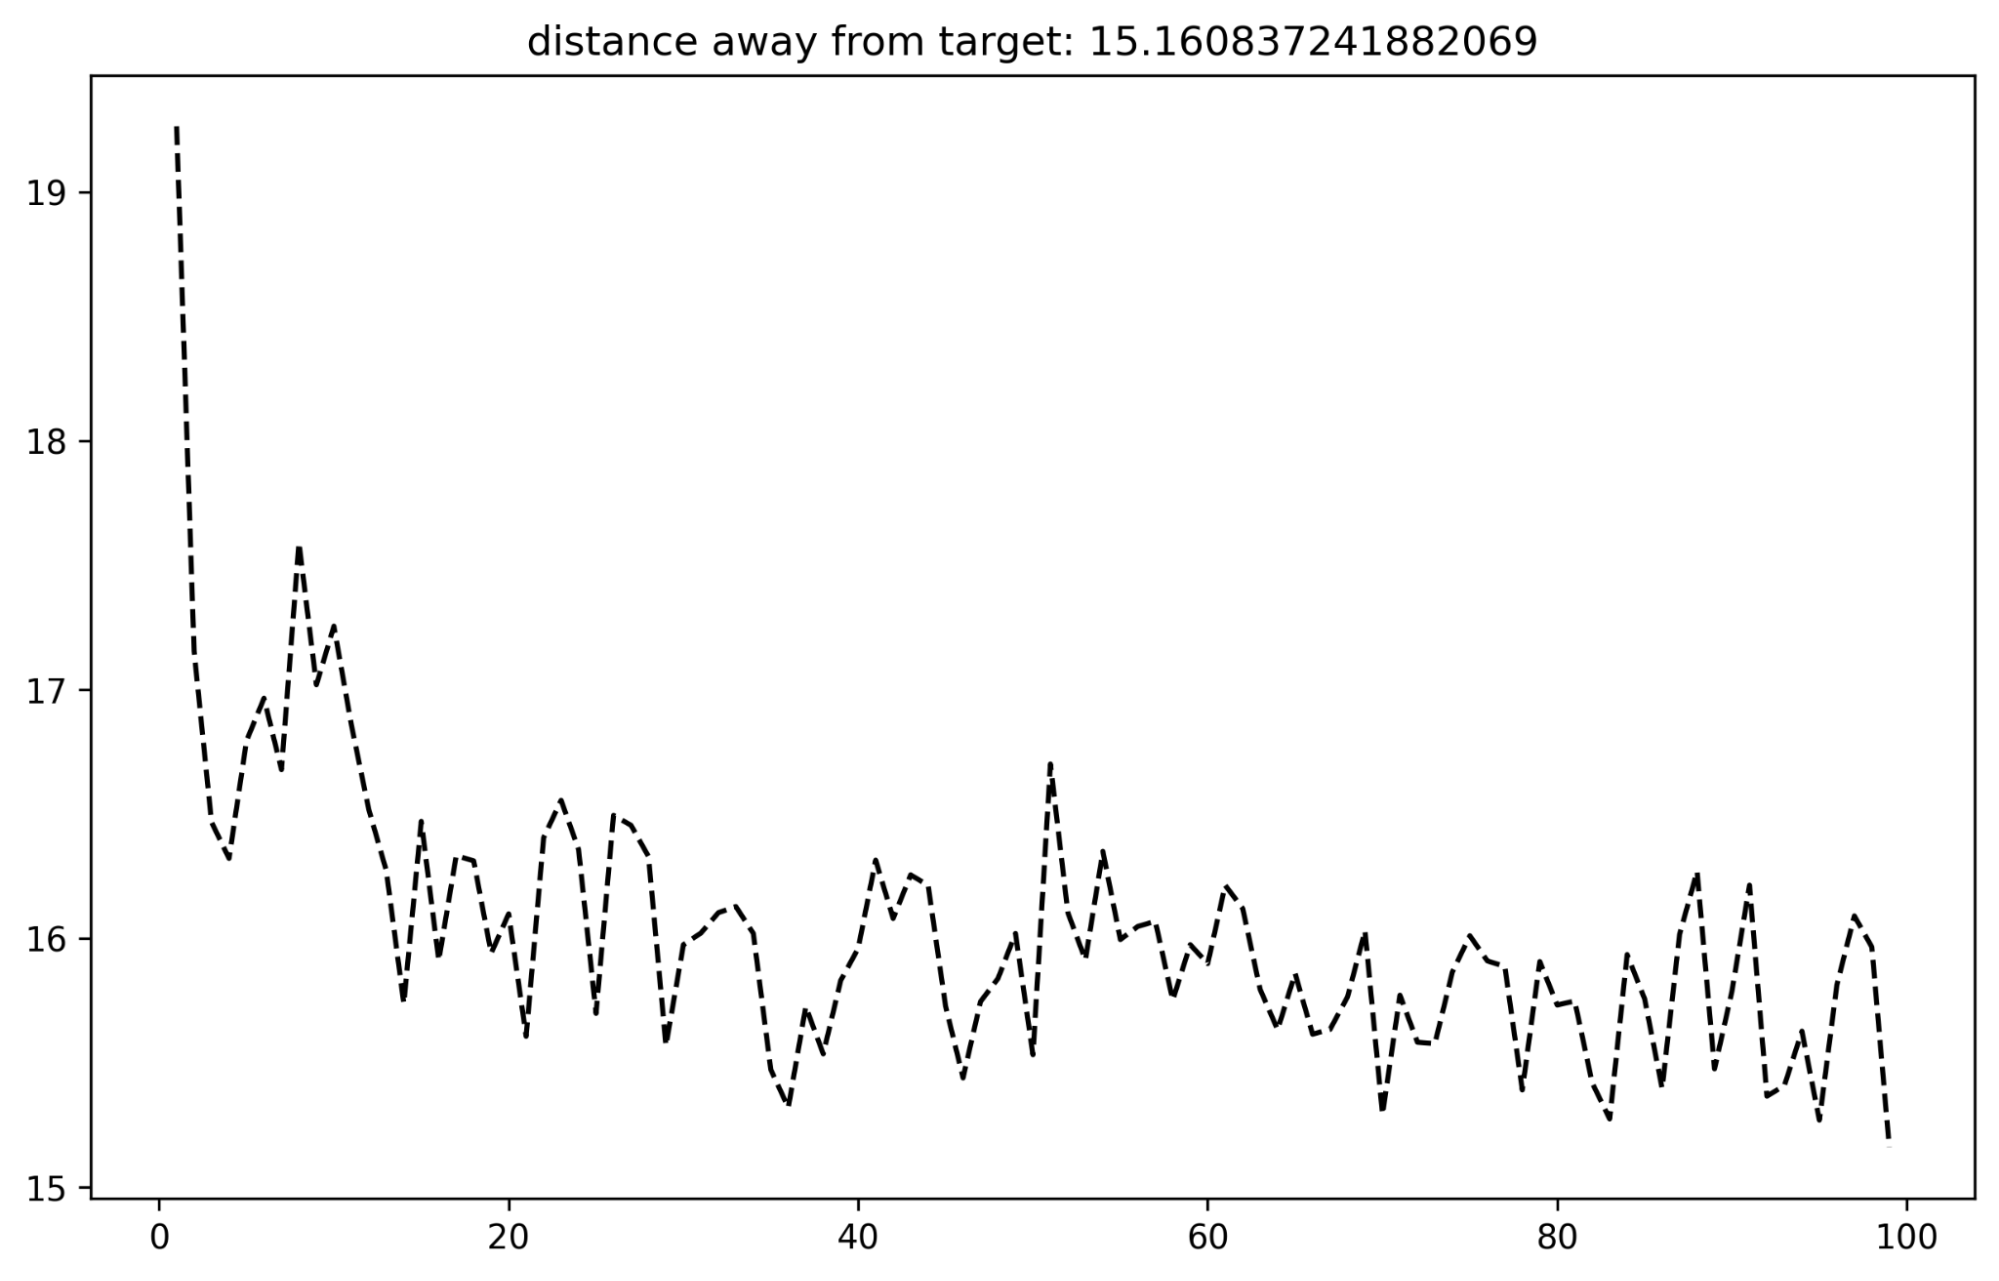
\includegraphics[width=\linewidth]{image4.png}
			\caption{RF Model AGT with BSSID filtering (1x1)}
			\label{fig:rf_agt_filter}
		\end{minipage}
		\hfill
		\begin{minipage}{0.45\textwidth}
			\centering
			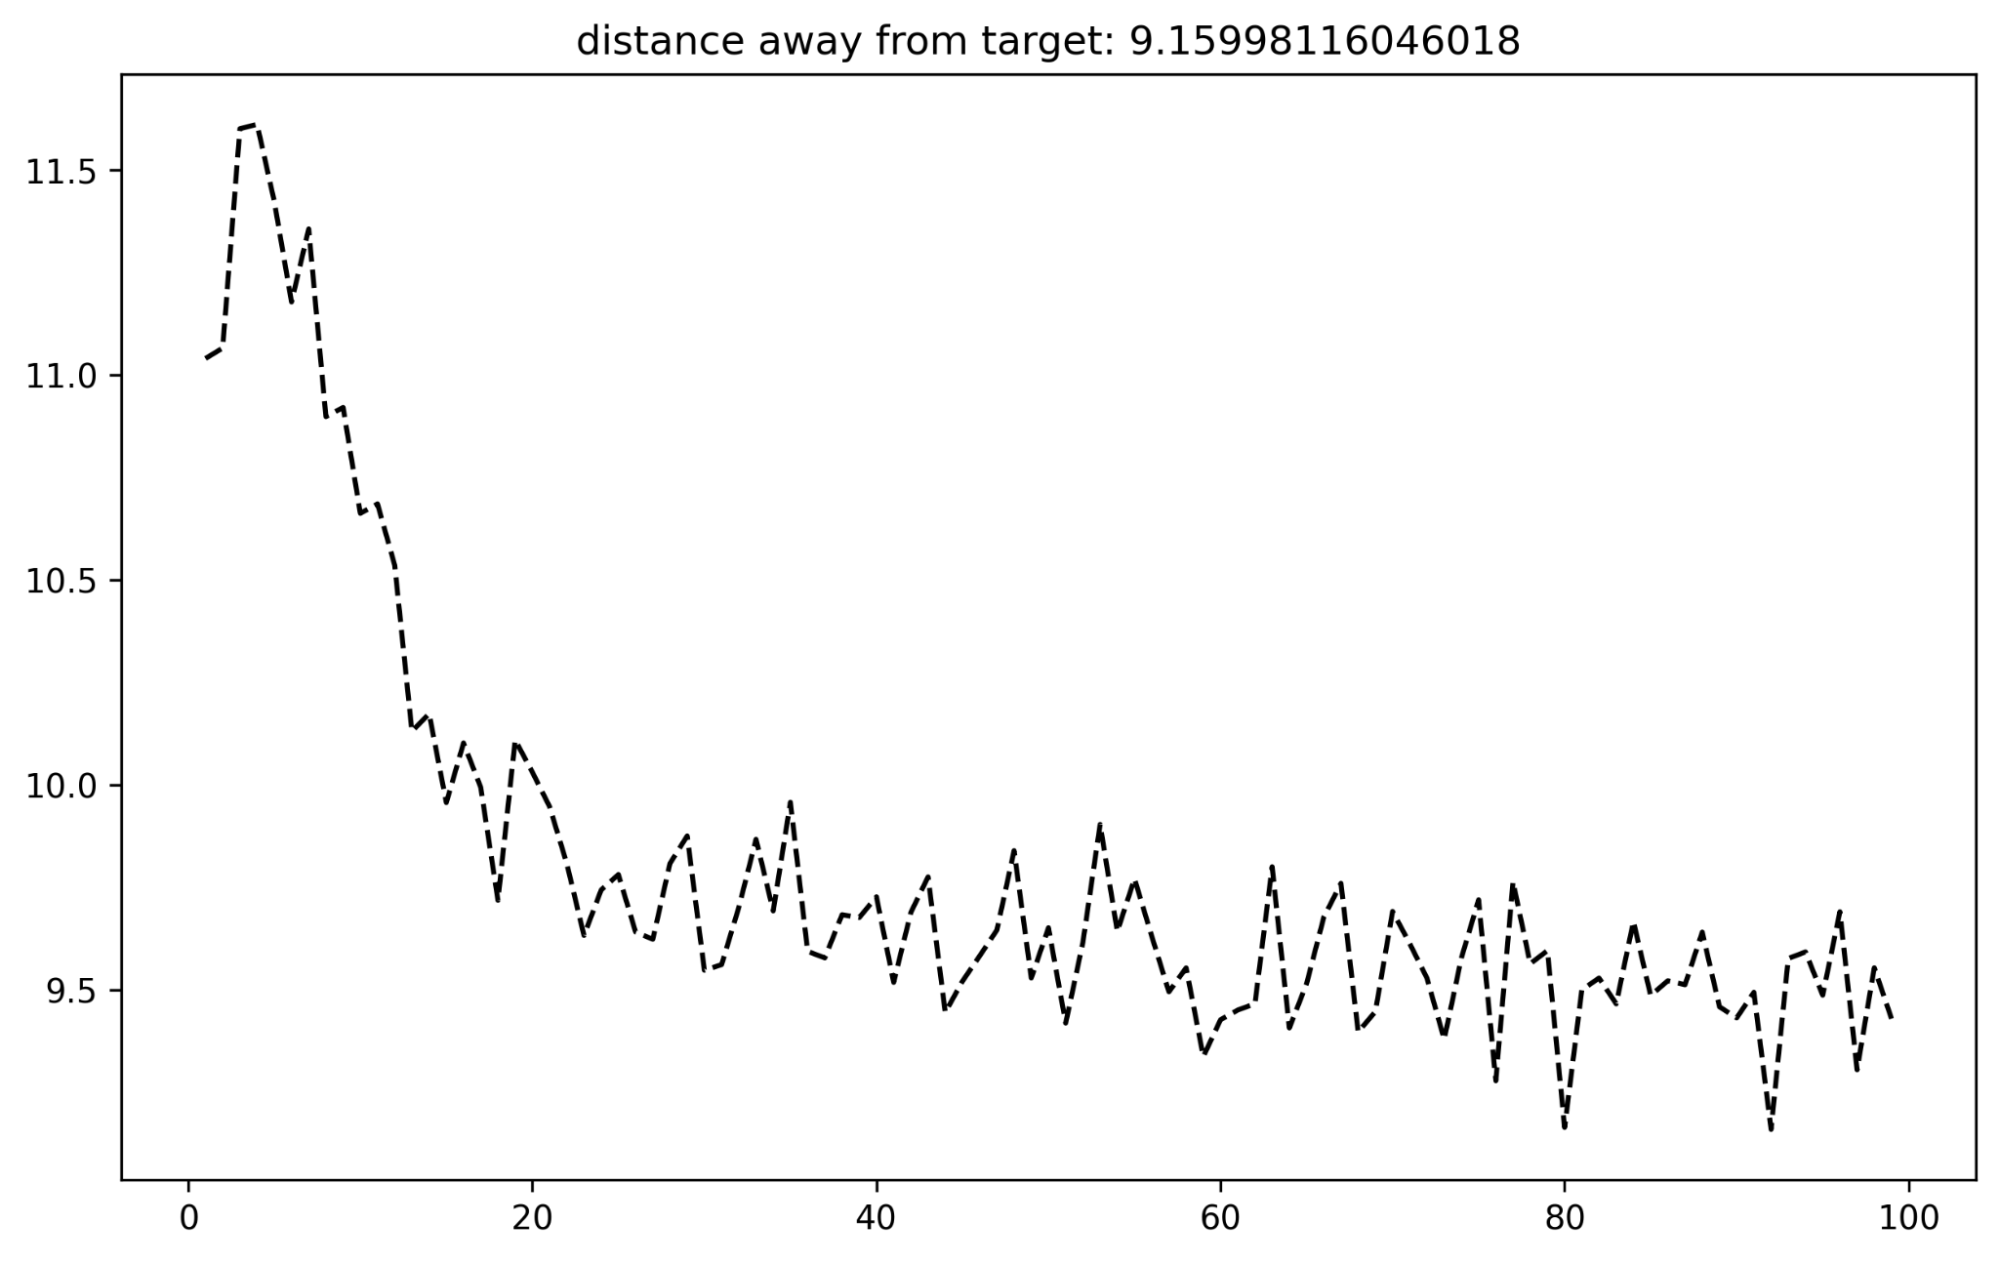
\includegraphics[width=\linewidth]{image7.png}
			\caption{RF Model AGT without BSSID filtering (1x1)}
			\label{fig:rf_agt_nofilter}
		\end{minipage}
	\end{figure*}
	
	\section{Discussion}
	By conducting our experiment across multiple grid sizes, we can visualize the tradeoff between grid size and precision. To quantify this, we calculate the average grid deviation from the target and multiply it by each grid size’s diagonal length, as shown in fig. \ref{fig:AGT_dgrid_size}. It illustrates the expected deviation in predictions when a model is trained on a specific grid size, should an error occur.
	
	While a 15×15m grid size performs well on the graph, it inherently limits accuracy to that resolution. In cases where predictions are correct, the location remains constrained within a 15×15m area, which may not be suitable for applications requiring higher precision—such as those needing to pinpoint areas smaller than this grid size.
	
	Through this experiment, we find that a 7×7m grid size offers the best balance between accuracy and precision. Below demonstrates our Average Distance away from Target metric (ADT) which is a byproduct between AGT and diagonal length of used grid size. Utilizing 7x7m grid size minimizes error while remaining small enough for use in precision-dependent applications. However, it is important to note that these findings may not generalize to all IPS implementations in different environments. The results suggest that increasing grid size does not necessarily improve accuracy or even precision; in some cases, performance actually declines, as shown in the chart. This highlights the need for careful consideration when selecting a grid size based on the specific requirements of an IPS deployment.
	
	
	\begin{figure}[htbp]
		\centerline{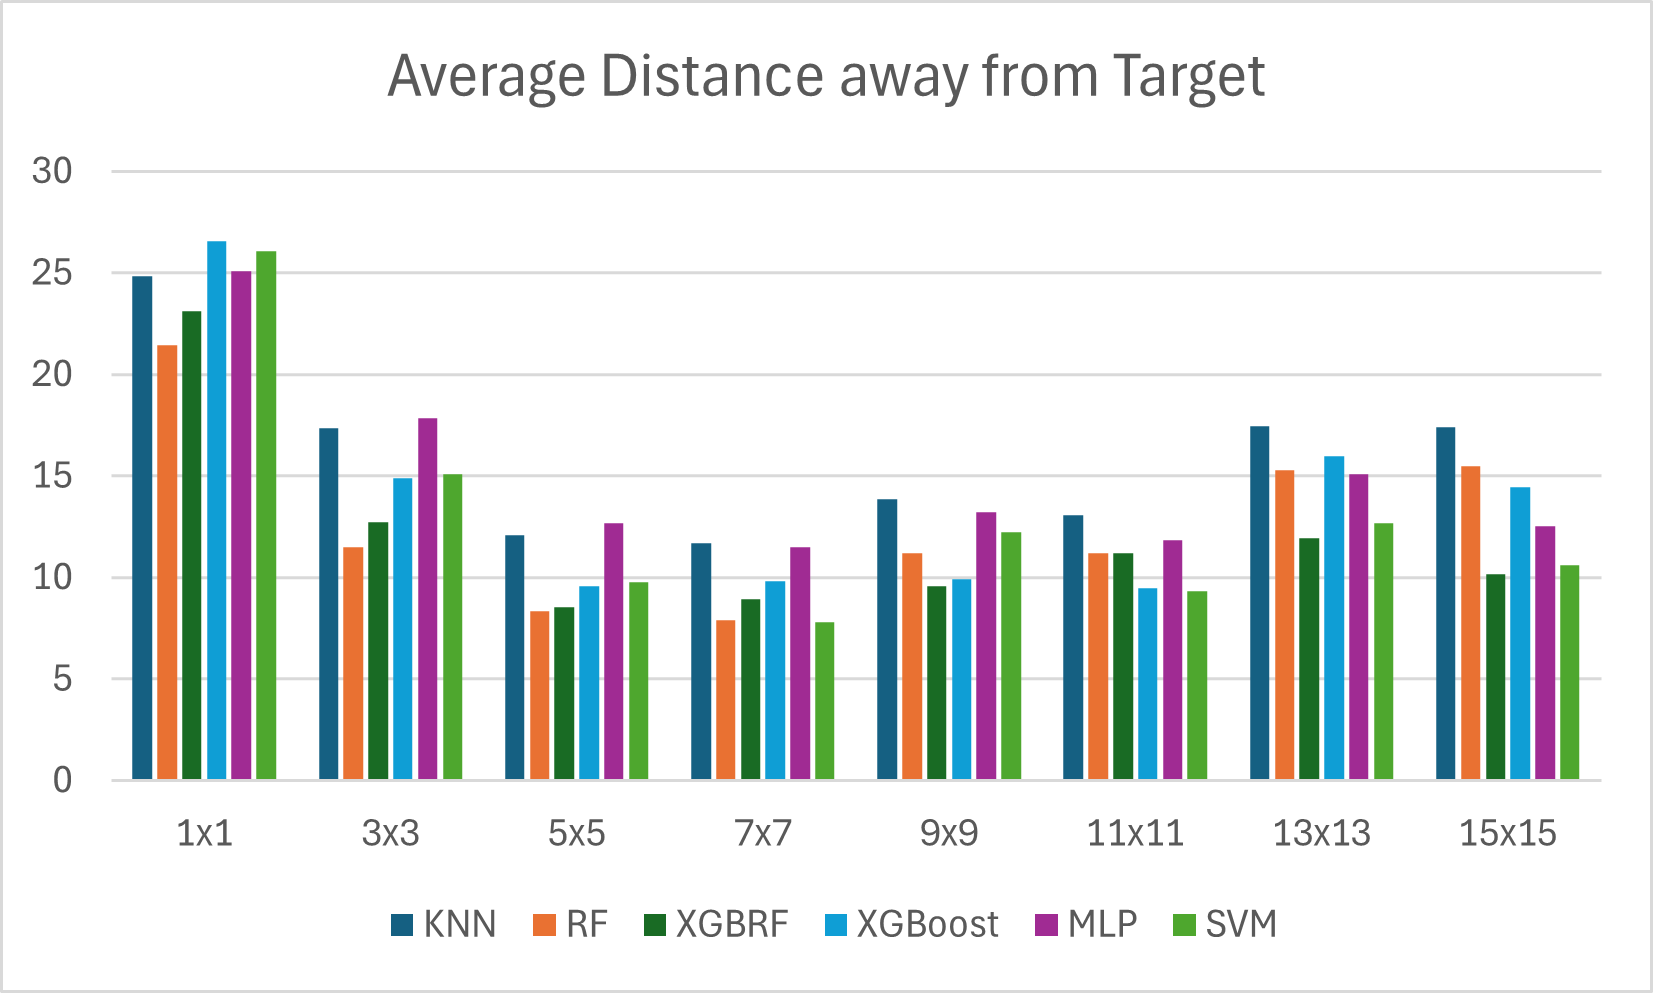
\includegraphics[scale=0.65]{image2.png}}
		\caption{Average Distance Error Across Different Grid Resolutions}
		\label{fig:Avg_dis_err}
	\end{figure}
	
	
	
	Training an IPS model involves significant computational challenges, particularly when dealing with high-dimensional feature spaces. In our experiment, we implemented a simple Wi-Fi access point filtering approach, selecting only access points containing specific identifiers in their names. This drastically reduced the number of access points used as features, making the training process more efficient.
	
	While the filtering method we applied was relatively simple, it had a surprisingly large impact on computational feasibility. Observing fig.~\ref{fig:rf_acc_filter} and~\ref{fig:rf_acc_nofilter}, by reducing the number of BSSID features from 1799 to 378, we were able to train models across a wide range of grid sizes (1×1 to 15×15) without overwhelming our hardware. In contrast, attempting to train on the full, unfiltered set quickly became impractical—our RTX 3080 Ti struggled even with the smallest grid size. Although we didn’t record exact runtimes, the difference in resource demands was stark. This raises questions about the actual utility of the full feature set and suggests that a more systematic study of feature selection or dimensionality reduction could be worthwhile in future works.
	
	Fig.~\ref{fig:rf_agt_filter} and~\ref{fig:rf_agt_nofilter} suggest that filtering access points did not negatively impact the model's learning process. A comparison of training trajectories for the 1×1 grid experiment shows that the filtered model performed comparably to the unfiltered one, if not slightly better in terms of convergence. This suggests that reducing feature dimensionality not only accelerates training but may also make learning more stable.
	
	

	
	
	
	\section{Conclusion}
	In conclusion, this paper extends our previous work by refining the implementation of an IPS using a classification-based approach. Through our experiments across multiple grid sizes, we visualized the trade-offs between grid size and precision, showing that increasing grid size does not necessarily improve accuracy and may, in some cases, lead to worse performance. Our findings suggest that a 7×7m grid size offers the best balance between accuracy and precision, making it suitable for applications that require finer localization. However, we acknowledge that these results may not generalize to all environments due to variations in WiFi signal behavior and building structures.
	
	Additionally, we implemented a simple filtering method to limit the number of WiFi BSSID features, preventing excessive model complexity while maintaining comparable performance to an unfiltered approach. This method significantly reduced training time and computational requirements, allowing us to complete model training across multiple grid sizes efficiently. Our results indicate that reducing feature dimensionality not only accelerates training but may also contribute to more stable learning. To better assess IPS performance, we introduced two new evaluation metrics—Average Grid from Target (AGT) and Average Distance from Target (ADT)—which provide a clearer understanding of prediction deviation. Ultimately, our study highlights key considerations in IPS design, particularly in grid size selection and feature filtering, and offers insights for improving indoor positioning accuracy in practical implementations.
	
	\begin{thebibliography}{00}
		\bibitem{bgp1} A, Nessa, B. Adhikari, F. Hussain and X. N. Fernando, A Survey of Machine Learning for Indoor Positioning," in IEEE Access, vol. 8, pp. 214945-214965, 2020, doi: 10.1109/ACCESS.2020.3039271
		\bibitem{bgp2} H. A. de Souza Mourão and H. A. B. F. de Oliveira, Indoor Localization System Using Fingerprinting and Novelty Detection for Evaluation of Confidence in Future Internet ,14(2) , 51. 2022, doi:  https://doi.org/10.3390/fi14020051 
		\bibitem{bgp3} H.T. Gidey, X. Guo, K. Zhong, L. Li, Y. Zhang. OHetTLAL: An Online Transfer Learning Method for Fingerprint-Based Indoor Positioning in  Sensors 2022, 22(23), 9044, doi: https://doi.org/10.3390/s22239044
		\bibitem{bgp4} H. Obeidat, W. Shuaieb, O. Obeidat, and R. Abd-Alhameed, "A Review of Indoor Localization Techniques and Wireless Technologies," *Wireless Personal Communications*, vol. 119, no. 1, pp. 289–327, Jul. 2021, doi: 10.1007/s11277-021-08209-5.
		\bibitem{bg2} D. Csik, Á. Odry, and P. Sarcevic, "Comparison of RSSI-Based Fingerprinting Methods for Indoor Localization," in *Proc. 20th IEEE International Symposium on Intelligent Systems and Informatics (SISY)*, Subotica, Serbia, Sep. 2022, pp. 000273–000278, doi: 10.1109/SISY56759.2022.10036270.
		\bibitem{LRE1} B. Intachuen, M. Charoenphon, T. Mankhetwit (2024), Classification-based-IPS [Online]. Available: \url{https://github.com/RinRin-32/Classification-based-IPS}
		\bibitem{LRE2} R. Vishwakarma, R. B. Joshi, and S. Mishra. IndoorGNN: A Graph Neural Network based approach for Indoor Localization using WiFi RSSI, In Big Data and Artificial Intelligence: 11th International Conference, BDA 2023, 150–165, \url{doi:https://doi.org/10.1007/978-3-031-49601-1_11}
		\bibitem{LRE3} D. Christodoulou,  Developing an indoor localisation and wayfinding app for a University Library Available: \url{https://project-archive.inf.ed.ac.uk/ug4/20223034/ug4_proj.pdf}
		\bibitem{LRE4} L. Bibbo, R. Carotenuto, F. D. Corte, An Overview of Indoor Localization System for Human Activity Recognition (HAR) in Healthcare in Sensors 22, no. 21: 8119, doi: \url{https://doi.org/10.3390/s22218119}
		\bibitem{LRE5}N. A. Maung Maung, B. Y. Lwi and S. Thida, "An Enhanced RSS Fingerprinting-based Wireless Indoor Positioning using Random Forest Classifier," 2020 International Conference on Advanced Information Technologies (ICAIT), Yangon, Myanmar, 2020, pp. 59-63, doi: 10.1109/ICAIT51105.2020.9261776.
		\bibitem{LRE6}P. Wongsekleo, L. Nakpaen, P. Cherntanomwong, and C. Pattiyanon, “Time Reduction for Collecting Fingerprint Data in Indoor Positioning Systems with Generated Synthetic Data by Ensemble Models and GANs”, in: Proc. 2024 19th International Joint Symposium on Artificial Intelligence and Natural Language Processing, Chonburi, Thailand, pp. 1–6, 610 2024. 
		\bibitem{LRE7}L. Nakpaen, P. Wongsekleo, P. Cherntanomwong, and C. Pattiyanon, “Building RSSI-based Indoor Positioning Fingerprint Maps using Android-based Coordination”, in: Proceedings of 2024 19th International Joint Symposium on Artificial Intelligence and Natural Language processing (iSAI-NLP), Chonburi, Thailand, pp. 1–6, 2024.
		
	\end{thebibliography}
	\vspace{12pt}
	\color{red}
	IEEE conference templates contain guidance text for composing and formatting conference papers. Please ensure that all template text is removed from your conference paper prior to submission to the conference. Failure to remove the template text from your paper may result in your paper not being published.
	
	
	\clearpage
	\begin{comment}
	\begin{figure*}[hbt!]
		\centering
		% Left Column (26XXXX IDs)
		\begin{minipage}{0.45\textwidth}
			\centering
			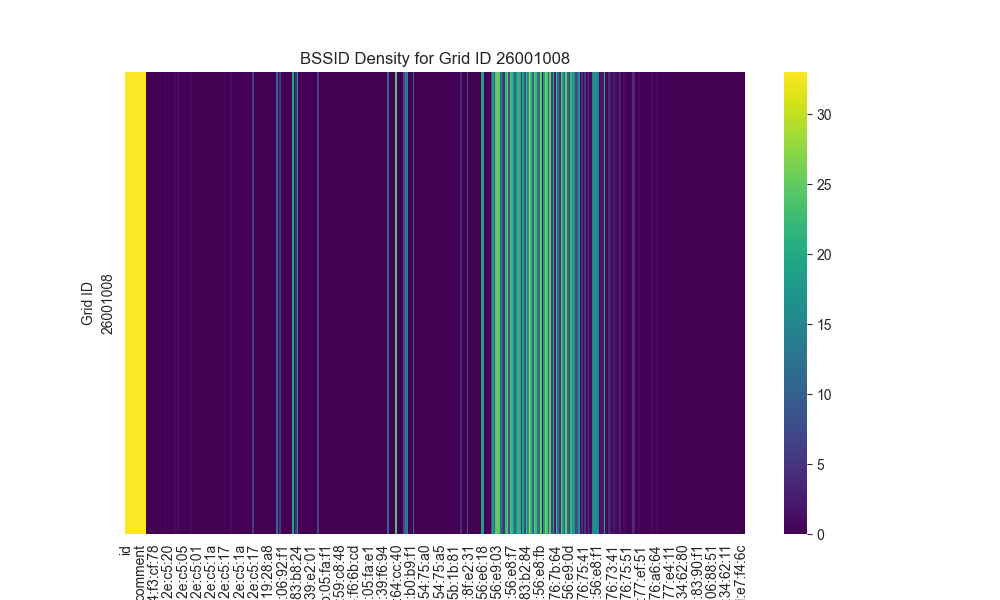
\includegraphics[width=1.25\linewidth]{heatmap_gridid_26001008.png}\par\medskip
			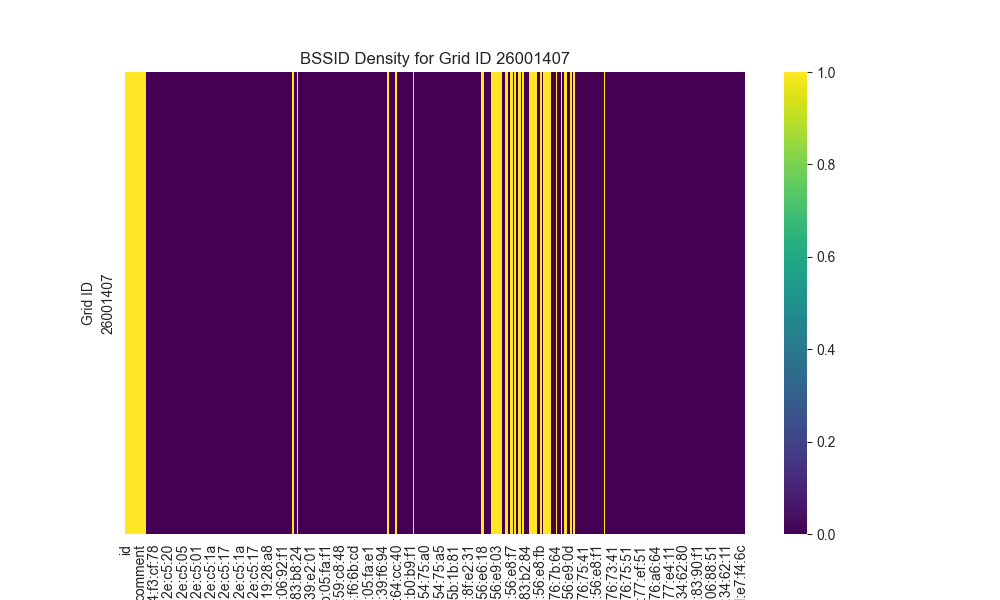
\includegraphics[width=1.25\linewidth]{heatmap_gridid_26001407.png}\par\medskip
			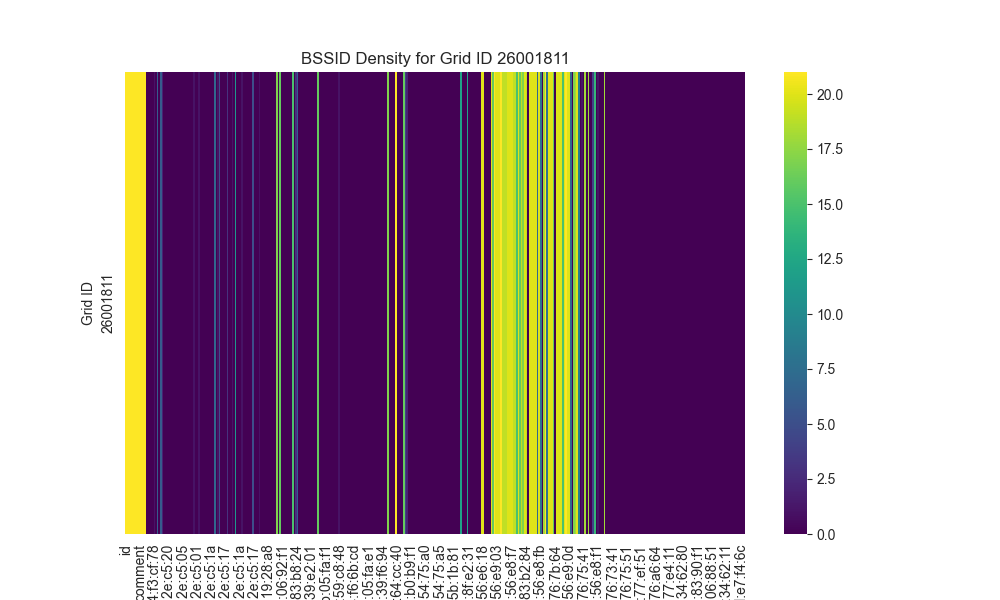
\includegraphics[width=1.25\linewidth]{heatmap_gridid_26001811.png}\par\medskip
			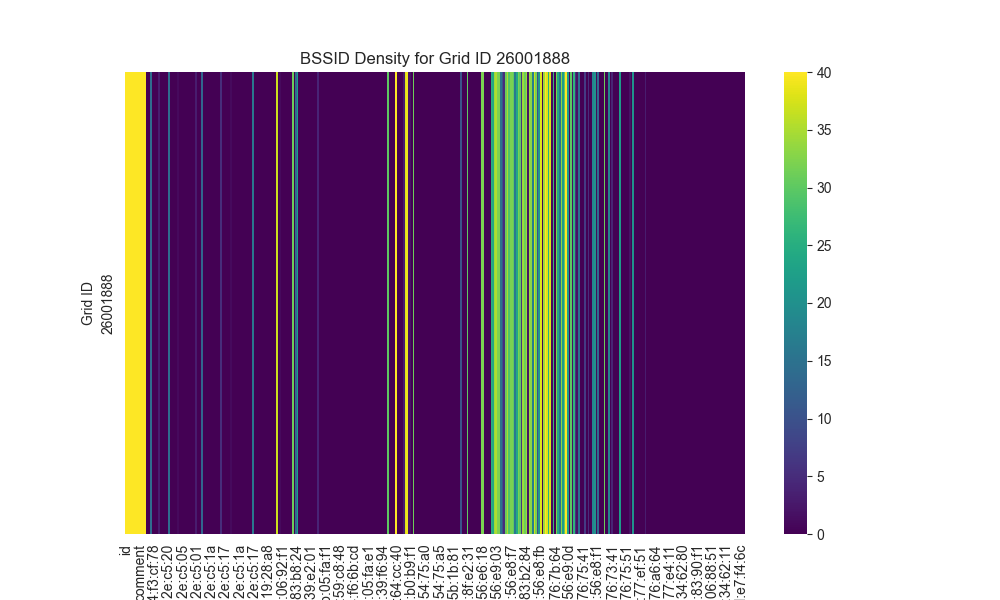
\includegraphics[width=1.25\linewidth]{heatmap_gridid_26001888.png}\par\medskip
			%\subfloat[Grid ID 260011369]{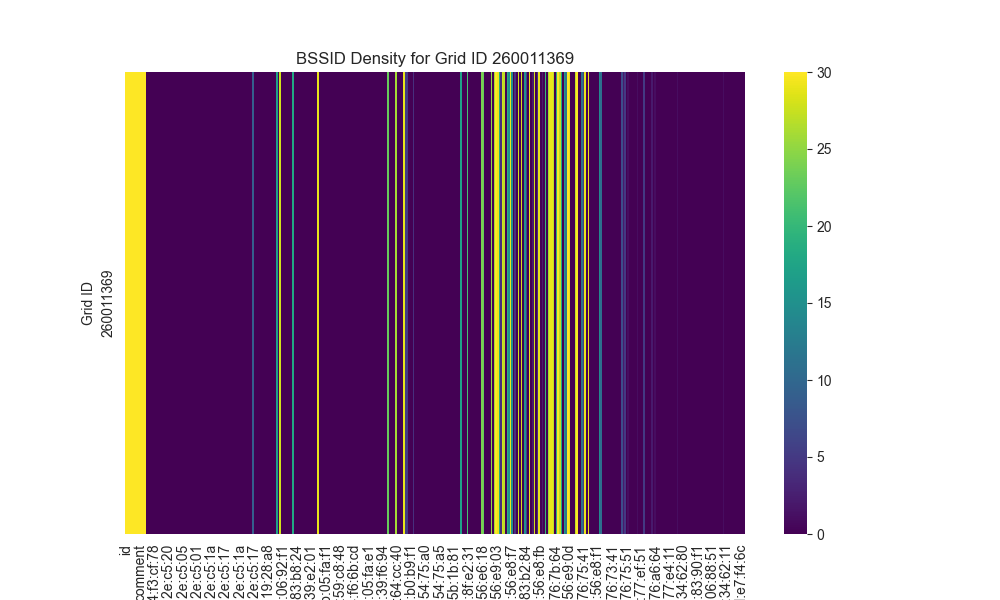
\includegraphics[width=1.25\linewidth]{heatmap_gridid_260011369.png}}
		\end{minipage}
		\hfill
		% Right Column (27XXXX IDs)
		\begin{minipage}{0.45\textwidth}
			\centering
			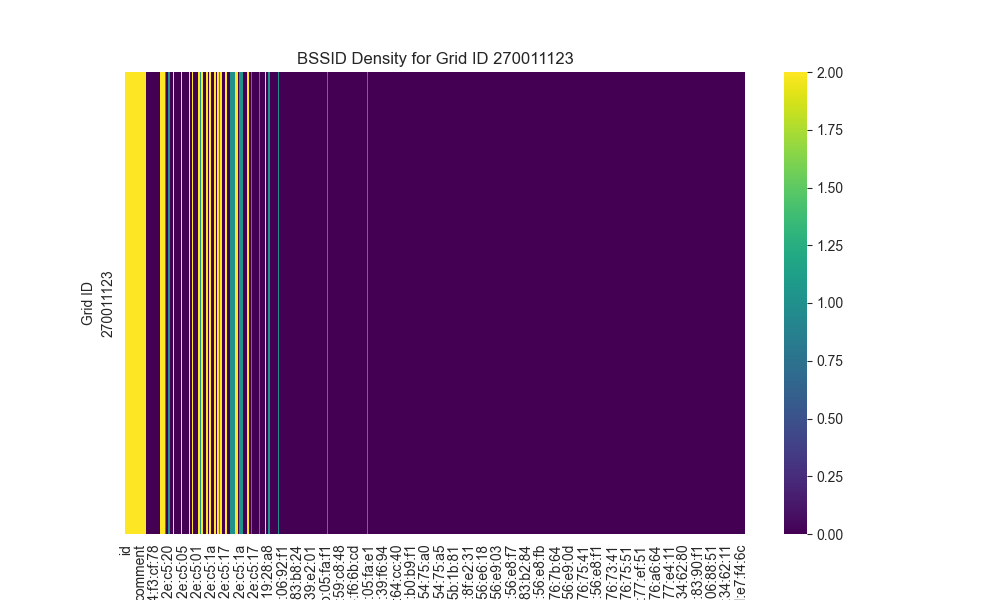
\includegraphics[width=1.25\linewidth]{heatmap_gridid_270011123.png}\par\medskip
			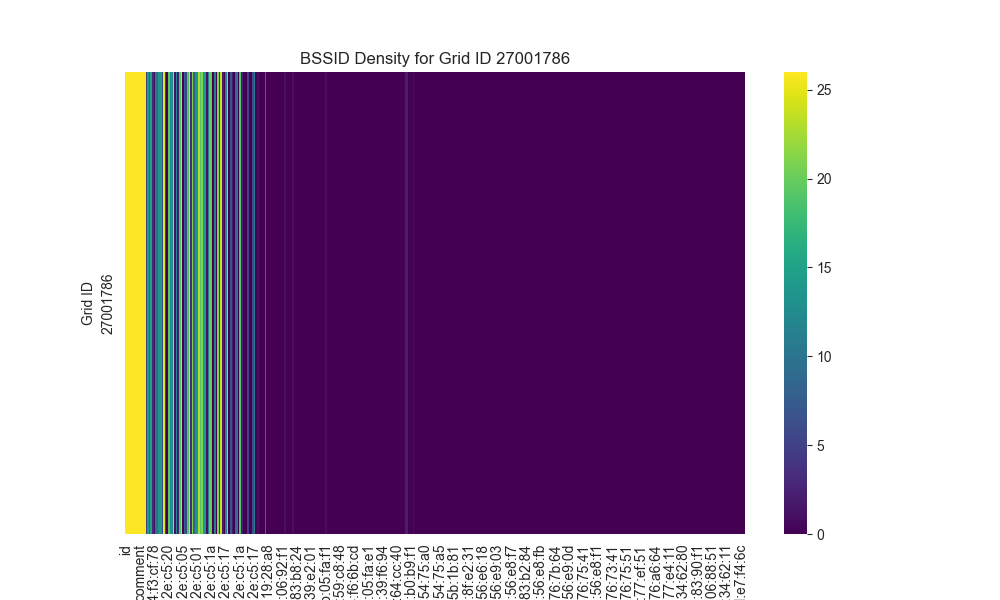
\includegraphics[width=1.25\linewidth]{heatmap_gridid_27001786.png}\par\medskip
			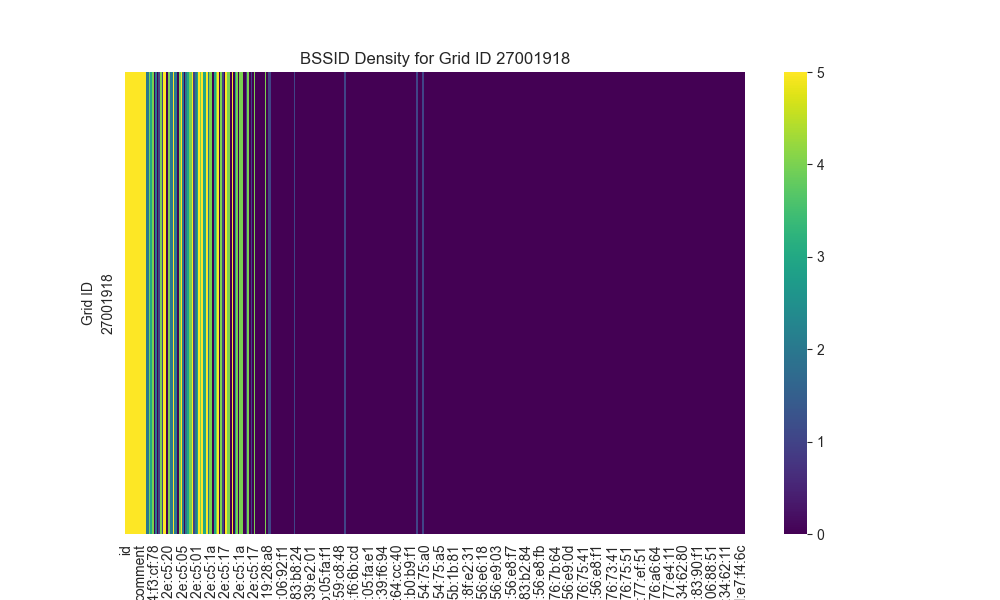
\includegraphics[width=1.25\linewidth]{heatmap_gridid_27001918.png}\par\medskip
			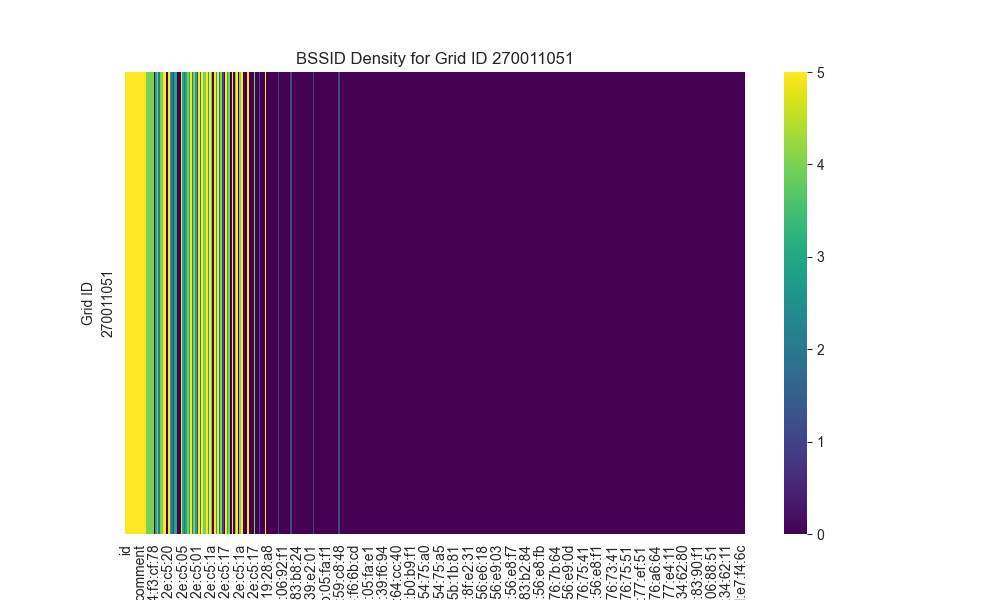
\includegraphics[width=1.25\linewidth]{heatmap_gridid_270011051.png}\par\medskip
			%\subfloat[Grid ID 270011105]{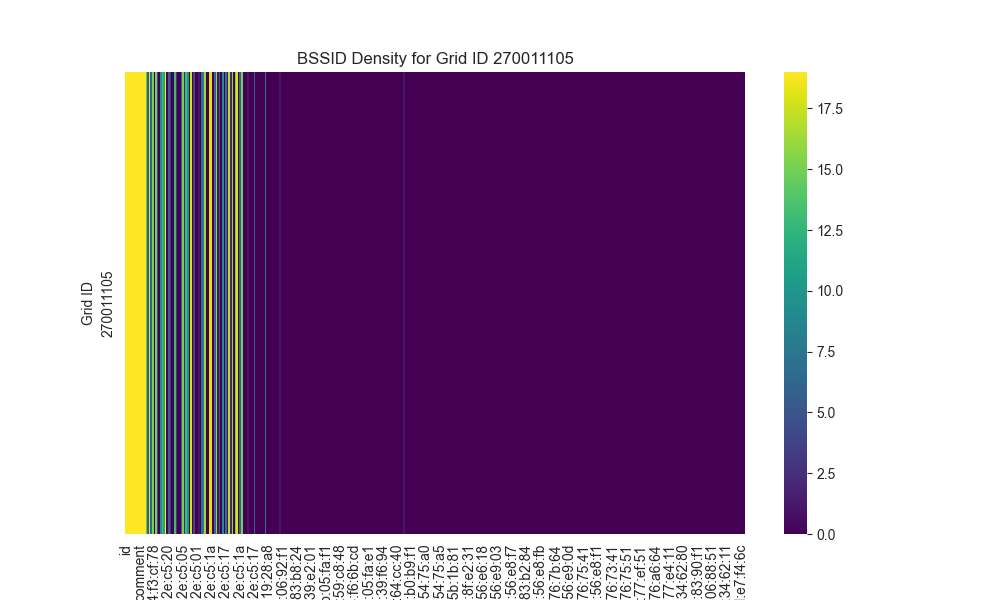
\includegraphics[width=1.25\linewidth]{heatmap_gridid_270011105.png}}
		\end{minipage}
		
		\caption{BSSID Heatmaps}
		\label{fig:bssid_heatmaps}
	\end{figure*}
	\end{comment}
\end{document}
